\def\booklet{0} % set to 1 to get a format for booklet printing
\ifodd\booklet
\documentclass[14pt]{extarticle}
\usepackage[margin=0.5in]{geometry}
\addtolength{\topmargin}{-.5in}
\addtolength{\textheight}{0.9in}
\else
\documentclass[11pt]{article}
\usepackage{marginnote}
%\usepackage[top=1in,bottom=1in,outer=2in,inner=1in,marginparsep=0.25in,
%marginparwidth=1.5in]{geometry}
\usepackage{fullpage}
\fi

\usepackage{amsfonts,amssymb,amsmath,amsthm,url,mathtools}
\usepackage{ifpdf}
\ifpdf
\usepackage[pdftex]{graphicx}
\else
\usepackage{graphicx}
\fi

\usepackage{fancyvrb}

\newcommand{\shaisays}[1]{$\ll$\textsf{#1 Shai}$\gg$}
\newcommand{\nigelsays}[1]{$\ll$\textsf{#1 Nigel}$\gg$}
\newcommand{\victorsays}[1]{\marginnote{\small V: #1}}

\newcommand{\ssum}[2]{\sum_{\substack{#1 \\ #2}}}

\newtheorem{lemma}{Lemma}
\newtheorem{theorem}{Theorem}

\newcommand{\defref}[1]{Definition~\protect\ref{def:#1}}
\newcommand{\secref}[1]{Section~\protect\ref{sec:#1}}
\newcommand{\appref}[1]{Appendix~\protect\ref{sec:#1}}
\newcommand{\figref}[1]{Figure~\protect\ref{fig:#1}}
\newcommand{\tblref}[1]{Table~\protect\ref{tbl:#1}}
\newcommand{\thmref}[1]{Theorem~\protect\ref{thm:#1}}
\newcommand{\lemref}[1]{Lemma~\protect\ref{lem:#1}}
\newcommand{\clmref}[1]{Claim~\protect\ref{clm:#1}}
\newcommand{\corref}[1]{Corollary~\protect\ref{cor:#1}}
\newcommand{\eqnref}[1]{Equation~(\protect\ref{eqn:#1})}

\newcommand{\A}{\mathbb{A}}
\newcommand{\B}{\mathbb{B}}
\newcommand{\C}{\mathbb{C}}
\newcommand{\F}{\mathbb{F}}
\newcommand{\GF}{\mathbb{GF}}
\newcommand{\hG}{\hat{\mathcal{G}}}
\newcommand{\K}{\mathbb{K}}
\renewcommand{\L}{\mathbb{L}}
\newcommand{\M}{\mathbb{M}}
\newcommand{\Q}{\mathbb{Q}}
%\newcommand{\R}{\mathbb{R}}
\newcommand{\Z}{\mathbb{Z}}
\newcommand{\N}{\mathbb{N}}

\def\Qct{Q_\mathsf{ct}}

\def\calA{\mathcal{A}}
\def\calB{\mathcal{B}}
\def\calE{\mathcal{E}}
\def\calP{\mathcal{P}}
\def\calS{\mathcal{S}}
\def\calQ{\mathcal{Q}}
\def\calU{\mathcal{U}}

\newcommand{\secparam}{\lambda}
\newcommand{\polylog}{\ensuremath{\textup{polylog}}}
\newcommand{\poly}{\ensuremath{\textup{poly}}}

\newcommand{\Gal}{\mathcal{G}\mathsf{al}}
\newcommand{\CRT}{\mathsf{CRT}}
\newcommand{\dCRT}{\mathsf{DoubleCRT}}

\newcommand{\grp}[1]{\left\langle #1 \right\rangle}
\def\ord{\mathsf{ord}}

\newcommand{\normI}[1]{\Vert #1 \Vert_\infty}
\newcommand{\normOne}[1]{\Vert #1 \Vert_1}
\newcommand{\normTwo}[1]{\Vert #1 \Vert_2}

\newcommand{\ceil}[1]{\left\lceil{#1}\right\rceil}
%\newcommand{\floor}[1]{\lfloor #1 \rfloor}
%\newcommand{\round}[1]{\lceil #1 \rfloor}
\newcommand{\vect}[1]{\left\langle{#1}\right\rangle}
\def\eqdef{\stackrel{\mathrm{def}}{=}}
\newcommand{\roundd}[1]{\Big\lceil #1 \Big\rfloor}

% Scheme Stuff

\def\NumbTh{\textsf{NumbTh}}
\def\bluestein{\textsf{bluestein}}
\def\PAlgebra{\textsf{PAlgebra}}
\def\PAlgebraTwo{\textbf{obsolete:PAlgebraTwo}}
\def\PAlgebraTwoR{\textbf{obsolete:PAlgebraTwoR}}
\def\PAlgebraMod{\textsf{PAlgebraMod}}
\def\Cmodulus{\textsf{Cmodulus}}
\def\IndexSet{\textsf{IndexSet}}
\def\IndexMap{\textsf{IndexMap}}
\def\SingleCRT{\textsf{SingleCRT}}
\def\DoubleCRT{\textsf{DoubleCRT}}
\def\FHE{\textsf{FHE}}
\def\Ctxt{\textsf{Ctxt}}
\def\KeySwitch{\textsf{KeySwitch}}
\def\FHEPubKey{\textsf{FHEPubKey}}
\def\FHESecKey{\textsf{FHESecKey}}
\def\SKHandle{\textsf{SKHandle}}
\def\CtxtPart{\textsf{CtxtPart}}
\def\FHEcontext{\textsf{FHEcontext}}
\def\EncryptedArray{\textsf{EncryptedArray}}
\def\EncryptedArrayModTwoR{\textbf{obsolete:EncryptedArrayModTwoR}}
\def\KeySwitching{\textsf{KeySwitching}}

\def\var#1{\ensuremath{\mathtt{#1}}}

\def\un{\texttt{\char"5F}}

\def\class{%
\begingroup\catcode`\_=12\relax
\classwitharg}

\def\classwitharg#1{\tt #1\endgroup}



\def\VAR{\mathsf{VAR}}
\def\EXP{\mathsf{E}}
\newcommand{\lev}{l}
\newcommand{\ql}{{q_{\lev}}}
\def\vr{\vec{r}}
\def\ve{\vec{e}}
\def\vc{\vec{c}}
\def\vd{\vec{d}}
\def\vs{\vec{s}}

\newcommand{\mfa}{\mathfrak{a}}
\newcommand{\mfb}{\mathfrak{b}}
\newcommand{\ee}{\mathfrak{e}}
\newcommand{\ct}{\mathfrak{c}}
\newcommand{\mm}{\mathfrak{m}}
\newcommand{\rr}{\mathfrak{r}}
\newcommand{\sk}{\mathfrak{s}}
\newcommand{\pk}{\mathfrak{pk}}

\newcommand{\Params}{\mathsf{Params}}
\newcommand{\KeyGen}{\mathsf{KeyGen}}
\newcommand{\Enc}{\mathsf{Enc}}
\newcommand{\Dec}{\mathsf{Dec}}
\newcommand{\Add}{\mathsf{Add}}
\newcommand{\Mult}{\mathsf{Mult}}
\newcommand{\nAdd}{\ell\mbox{-}\Add}
\newcommand{\nMult}{\ell\mbox{-}\Mult}

\newcommand{\Swap}{\mathsf{Swap}}
\newcommand{\Select}{\mathsf{Select}}
\newcommand{\Selects}{\mathsf{Select}\textup{s}}
\newcommand{\SwitchKey}{\ensuremath{\mathsf{SwitchKey}}}
\newcommand{\SwitchModulus}{\ensuremath{\mathsf{SwitchModulus}}}
\newcommand{\Conjugate}{\mathsf{Conjugate}}
\newcommand{\CoeffExtract}{\mathsf{CoeffExtract}}
\newcommand{\CoeffPack}{\mathsf{CoeffPack}}
\newcommand{\Permute}{\mathsf{Permute}}
\newcommand{\nPermute}{\ell\mbox{-}\Permute}
\newcommand{\BitDecomp}{\ensuremath{{\mathsf{BitDecomp}}}}
\newcommand{\HomBitDecomp}{\ensuremath{{\mathsf{HomBitDecomp}}}}
\newcommand{\Refresh}{\ensuremath{{\mathsf{Refresh}}}}
\newcommand{\PowersTwo}{\ensuremath{{\mathsf{Powersof2}}}}
\newcommand{\Clone}{\ensuremath{{\mathsf{Clone}}}}
\newcommand{\nClone}{\ell\mbox{-}\Clone}
\newcommand{\Frobenius}{\ensuremath{{\mathsf{Frobenius}}}}
\newcommand{\nFrobenius}{\ell\mbox{-}\Frobenius}
\newcommand{\Scale}{\ensuremath{{\mathsf{Scale}}}}
\newcommand{\Pack}{\ensuremath{{\mathsf{Pack}}}}
\newcommand{\Unpack}{\ensuremath{{\mathsf{Unpack}}}}

%%%%%%%%%%%%%%%%%%%%%%%%%%%%%%%%%%%%%%%%%%%%%%%%%%%%%%%%%%%%%%%%%%%%%%
%%%%%%%%%%%%%%%%%%%%%%%%%%%%%%%%%%%%%%%%%%%%%%%%%%%%%%%%%%%%%%%%%%%%%%
%%%%%%%%%%%%%%%%%%%%%%%%%%%%%%%%%%%%%%%%%%%%%%%%%%%%%%%%%%%%%%%%%%%%%%
\begin{document}
\sloppy % VJS: I always use this to avoid things getting pushed
        % into the margin, which I find much worse than
        % extra spacing

\pagestyle{empty}
\begin{titlepage}
\title{Design and Implementation of a Homomorphic-Encryption Library}
\author{Shai Halevi \and Victor Shoup}
\maketitle

\begin{abstract}
We describe the design and implementation of a software library that
implements the Brakerski-Gentry-Vaikuntanathan (BGV) homomorphic
encryption scheme, along with many optimizations to make homomorphic
evaluation runs faster, focusing mostly on effective use of the
Smart-Vercauteren ciphertext packing techniques. Our library is
written in C++ and uses the NTL mathematical library. It is distributed
under the terms of the GNU General Public License (GPL).
\end{abstract}

\bigskip\bigskip\noindent
Partially supported by DARPA under agreement number
FA8750-11-C-0096. The U.S. Government is authorized to reproduce and
distribute reprints for Governmental purposes notwithstanding any
copyright notation thereon. The views and conclusions contained herein
are those of the authors and should not be interpreted as necessarily
representing the official policies or endorsements, either expressed
or implied, of DARPA or the U.S. Government. 
Distribution Statement ``A'' (Approved for Public Release,
Distribution Unlimited).

Also partially supported by the Intelligence Advanced Research
Projects Activity (EARP) via Department of Interior National Business
Center (DoI/NBC) contract number D11PC20202. The U.S. Government is
authorized to reproduce and distribute reprints for Governmental
purposes notwithstanding any copyright annotation thereon. Disclaimer:
The views and conclusions contained herein are those of the authors
and should not be interpreted as necessarily representing the official
policies or endorsements, either expressed or implied, of IARPA,
DoI/NBC, or the U.S. Government.
\end{titlepage}

\tableofcontents
\newpage
\pagestyle{plain}
\setcounter{page}1

\section*{Organization of This Report}
We begin in \secref{BGV} with a brief high-level overview of the
BGV cryptosystem and some important features of the variant that we
implemented and our choice of representation, as well as an overview
of the structure of our library. Then in Sections~\ref{sec:math},
\ref{sec:crypto},\ref{sec:dataMove} we give a bottom-up detailed
description of all the modules in the library. We conclude in
\secref{using} with some examples of using this library.

%%%%%%%%%%%%%%%%%%%%%%%%%%%%%%%%%%%%%%%%%%%%%%%%%%%%%%%%%%%%%%%%%%%%%%
\section{The BGV Homomorphic Encryption Scheme} \label{sec:BGV}
%%%%%%%%%%%%%%%%%%%%%%%%%%%%%%%%%%%%%%%%%%%%%%%%%%%%%%%%%%%%%%%%%%%%%%
A homomorphic encryption scheme \cite{RivestAD78,Gentry09} allows
processing of
encrypted data even without knowing the secret decryption key. In this
report we describe the design and implementation of a software library
that implements the Brakerski-Gentry-Vaikuntanathan (BGV)
homomorphic encryption scheme \cite{BGV12}. We begin by a high-level
description of the the BGV variant that we implemented, followed by
a detailed description of the various software components in our
implementation. 
The description in this section is mostly taken from
the full version of~\cite{GHS12c}.

Below we denote by $[\cdot]_q$ the reduction-mod-$q$ function, namely
mapping an integer $z\in\Z$ to the unique representative of its
equivalence class modulo~$q$ in the interval $(-q/2,q/2]$. We use
the same notation for modular reduction of vectors, matrices, etc.

Our BGV variant is defined over polynomial rings of the form
$\A=\Z[X]/\Phi_m(X)$ where $m$ is a parameter and $\Phi_m(X)$ is
the $m$'th cyclotomic polynomial. The ``native'' plaintext space for
this scheme is usually the ring $\A_2=\A/2\A$, namely binary polynomials
modulo $\Phi_m(X)$. (Our implementation supports other plaintext
spaces as well, but in this report we mainly describe the case of
plaintext space~$\A_2$. See some more details in \secref{PAlgebra}.)
We use the Smart-Vercauteren CRT-based encoding technique \cite{SV11}
to ``pack'' a vector of bits in a binary polynomial, so that
polynomial arithmetic in~$\A_2$ translates to entry-wise arithmetic on
the packed bits.

The ciphertext space for this scheme consists of vectors over
$\A_q=\A/q\A$, where $q$ is an
odd modulus that evolves with the homomorphic evaluation. Specifically,
the system is parametrized by a ``chain'' of moduli of decreasing size,
$q_0< q_1< \cdots <q_L$ and freshly encrypted ciphertexts
are defined over~$R_{q_L}$. During homomorphic evaluation we keep
switching to smaller and smaller moduli until we get ciphertexts
over~$\A_{q_0}$, on which we cannot compute anymore. We call
ciphertexts that are defined over~$\A_{q_i}$ ``level-$i$
ciphertexts''. These level-$i$ ciphertexts are 2-element vectors
over $R_{q_i}$, i.e., $\vc=(c_0,c_1)\in (\A_{q_i})^2$.

Secret keys are polynomials $\sk\in\A$ with ``small'' coefficients,
and we view $\sk$ as the second element of the 2-vector $\vs=(1,\sk)$.
A level-$i$ ciphertext $\vc=(c_0,c_1)$ encrypts a plaintext polynomial
$m\in \A_2$ with respect to $\vs=(1,\sk)$ if we have the equality over
$\A$, $[\vect{\vc,\vs}]_{q_i} = [c_0 + \sk \cdot c_1]_{q_i} \equiv m
\pmod{2}$, and moreover the polynomial $[c_0 + \sk \cdot c_1]_{q_i}$
is ``small'', i.e. all its coefficients are considerably smaller than
$q_i$. Roughly, that polynomial is considered the ``noise'' in the
ciphertext, and its coefficients grow as homomorphic operations are
performed. We note that the crux of the noise-control technique from
\cite{BGV12} is that a level-$i$ ciphertext can be publicly converted
into a level-$(i+1)$ ciphertext (with respect to the same secret key),
and that this transformation reduces the noise in the ciphertext
roughly by a factor of $q_{i+1}/q_i$.

Following \cite{LPR10,GHS12a,GHS12c}, we think of the ``size'' of a
polynomial $a\in\A$ as the norm of its canonical embedding. Recall that
the canonical embedding of $a\in\A$ into $\C^{\phi(m)}$ is the
$\phi(m)$-vector of complex numbers $\sigma(a)=(a(\tau_m^j))_j$
where $\tau_m$ is a complex primitive $m$-th root of unity
$(\tau_m=e^{2\pi i/m})$ and the indexes~$j$ range over all of
$\Z_m^*$. We denote the $l_2$-norm of the canonical embedding
of~$a$ by $\|a\|_2^{\mathrm{canon}}$.

The basic operations that we have in this scheme are the usual
key-generation, encryption, and decryption, the homomorphic evaluation
routines for addition, multiplication and automorphism (and also
addition-of-constant and multiplication-by-constant), and the
``ciphertext maintenance'' operations of key-switching and
modulus-switching. These are described in the rest of this report,
but first we describe our plaintext encoding conventions and our
Double-CRT representation of polynomials.

%%%%%%%%%%%%%%%%%%%%%%%%%%%%%%%%%%%%%%%%%%%%%%%%%%%%%%%%%%%%%%%%%%%%%%
\subsection{Plaintext Slots} \label{sec:slots}
The native plaintext space of our variant of BGV are elements of
$\A_2$, and the polynomial $\Phi_m(X)$ factors modulo~2 into $\ell$
irreducible factors, $\Phi_m(X)=F_1(X)\cdot F_2(X) \cdots F_{\ell}(X)
\pmod 2$, all of degree $d=\phi(m)/\ell$.
Just as in \cite{BGV12,GHS12a,SV11} each factor corresponds to a
``plaintext slot''. That is, we can view a polynomial $a\in\A_2$ as
representing an $\ell$-vector $(a\bmod F_i)_{i=1}^{\ell}$.

More specifically, for the purpose of packing we think of a
polynomial $a\in\A_2$ not as a binary polynomial but as a
polynomial over the extension field~$\F_{2^d}$ (with some specific
representation of that field), and the plaintext values that are
encoded in~$a$ are its evaluations at $\ell$ specific primitive
$m$-th roots of unity in $\F_{2^d}$.
In other words, if $\rho\in\F_{2^d}$ is a
particular fixed primitive $m$-th root of unity, and our distinguished
evaluation points are $\rho^{t_1},\rho^{t_2},\ldots,\rho^{t_{\ell}}$
(for some set of indexes $T=\{t_1,\ldots,t_\ell\}$), then the vector
of plaintext values encoded in~$a$ is:
\[
\big(a(\rho^{t_j})~:~ t_j \in T\big).
\]
See \secref{PAlgebra} for a discussion of the choice of representation
of $\F_{2^d}$ and the evaluation points.

It is a standard fact that (for an abstract primitive $m$-th root of
unity~$\zeta_m$), the Galois group $\Gal=\Gal(\Q(\zeta_m)/\Q)$
consists of the mappings $\kappa_k: a(X)\mapsto a(X^k)\bmod\Phi_m(X)$
for all $k$ co-prime with~$m$, and that it is isomorphic to $\Z_m^*$.
As noted in \cite{GHS12a}, for each $i,j\in\{1,2,\ldots,\ell\}$ there
is an element $\kappa_k\in\Gal$ which sends an element in slot~$i$ to
an element in slot~$j$. Indeed if we set $k=t_j^{-1}\cdot t_i\pmod m$
and $b = \kappa_k(a)$ then we have
\[
b(\rho^{t_j}) = a(\rho^{t_jk}) = a(\rho^{t_j\cdot t_j^{-1} t_i})
= a(\rho^{t_i}),
\]
so the element in the $j$'th slot of~$b$ is the same as that in the
$i$'th slot of~$a$.
In addition to these ``data-movement maps'', $\Gal$ contains also the
Frobenius maps, $X \longrightarrow X^{2^i}$, which also act as
Frobenius on the individual slots.

We note that the values that are encoded in the slots do not have to
be individual bits, in general they can be elements of the extension
field $\F_{2^d}$ (or any sub-field of it). For example, for the AES
application we may want to pack elements of $\F_{2^8}$ in the slots,
so we choose the parameters so that $\F_{2^8}$ is a sub-field of
$\F_{2^d}$ (which means that $d$ is divisible by~8).


More generally, we allow plaintext spaces of the form $\A_{p^r}$,
rather than just $\A_2$, where $p$ is an arbitrary prime (which does 
not divide $m$) and $r$ is a small positive integer.
In this setting, $\Phi_m(X)$ factors as $\prod_{i=1}^\ell F_i$
modulo $\Z_{p^r}$, where each $F_i$ is irreducible modulo $p^r$ 
of the same
degree $d$.
Note that in the case $r > 1$, the factorization of $\Phi_m(X)$
is determined by Hensel lifting.
The $i$th plaintext slot is isomorphic as a $\Z_{p^r}$-algebra to $\Z_{p^r}/(F_i)$.
It turns out that all these different rings are isomorphic ---
in the case where $r = 1$, they are isomorphic to the
finite field $\F_{p^d}$.

%%%%%%%%%%%%%%%%%%%%%%%%%%%%%%%%%%%%%%%%%%%%%%%%%%%%%%%%%%%%%%%%%%%%%%
\subsection{Our Modulus Chain and Double-CRT Representation}
\label{sec:dcrt}
We define the chain of moduli by choosing $L+1$ ``small primes'' $p_0,
p_1,\ldots,p_{L}$ and the $\lev$'th modulus in our chain is defined
as $\ql=\prod_{j=0}^\lev p_j$. 
The primes $p_i$'s are chosen so that
for all~$i$, $\Z/p_i\Z$ contains a primitive $m$-th root of unity
(call it $\zeta_i$) so $\Phi_m(X)$ factors modulo~$p_i$ to linear
terms $\Phi_m(X)= \prod_{j\in\Z_m^*} (X-\zeta_i^j)\pmod{p_i}$.

A key feature of our implementation is that we represent an element
$a\in\A_\ql$ via double-CRT representation, with respect to both the
integer factors of~$\ql$ and the polynomial factors of $\Phi_m(X)$
mod~$\ql$. A polynomial $a\in\A_q$ is represented as the $(\lev+1)
\times \phi(m)$ matrix of its evaluation at the roots of $\Phi_m(X)$
modulo $p_i$ for $i=0,\ldots,\lev$:
\[\dCRT^\lev(a) = \left(
  a(\zeta_i^j)\bmod p_i \right)_{0\le i\le\lev,~ j\in\Z_m^*}.
\]

Addition and multiplication in $\A_q$ can be computed as component-wise
addition and multiplication of the entries in the two tables (modulo
the appropriate primes~$p_i$),
\begin{eqnarray*}
   \dCRT^\lev(a+b) &=& \dCRT^\lev(a)+\dCRT^\lev(b),\\
   \dCRT^\lev(a \cdot b) &=& \dCRT^\lev(a) \cdot \dCRT^\lev(b). 
\end{eqnarray*}
Also, for an element of the Galois group $\kappa\in\Gal$, mapping
$a(X)\in\A$ to $a(X^k)\bmod\Phi_m(X)$, we can evaluate $\kappa(a)$
on the double-CRT representation of~$a$ just by permuting the columns
in the matrix, sending each column $j$ to column $j\cdot k \bmod m$.

%%%%%%%%%%%%%%%%%%%%%%%%%%%%%%%%%%%%%%%%%%%%%%%%%%%%%%%%%%%%%%%%%%%%%%
\subsection{Modules in our Library} \label{sec:modules}
Very roughly, our HE library consists of four layers: in the bottom
layer we have modules for implementing mathematical structures and
various other utilities, the second layer implements our Double-CRT
representation of polynomials, the third layer implements the
cryptosystem itself (with the ``native'' plaintext space of binary
polynomials), and the top layer provides interfaces for using the
cryptosystem to operate on arrays of plaintext values (using the
plaintext slots as described in \secref{slots}). We think of the
bottom two layers as the ``math layers'', and the top two layers
as the ``crypto layers'', and describe then in detail in Sections
\ref{sec:math} and~\ref{sec:crypto}, respectively. A block-diagram
description of the library is given in \figref{blocks}. Roughly,
the modules {\NumbTh}, \texttt{timing}, {\bluestein}, {\PAlgebra},
{\PAlgebraMod}, {\Cmodulus}, {\IndexSet} and
{\IndexMap} belong to the bottom layer,  {\FHEcontext}, {\SingleCRT}
and {\DoubleCRT} belong to the second layer, {\FHE}, {\Ctxt} and
{\KeySwitching} are in the third layer, and {\EncryptedArray} 
is in the top layer.

\begin{figure}
\ifpdf
\centerline{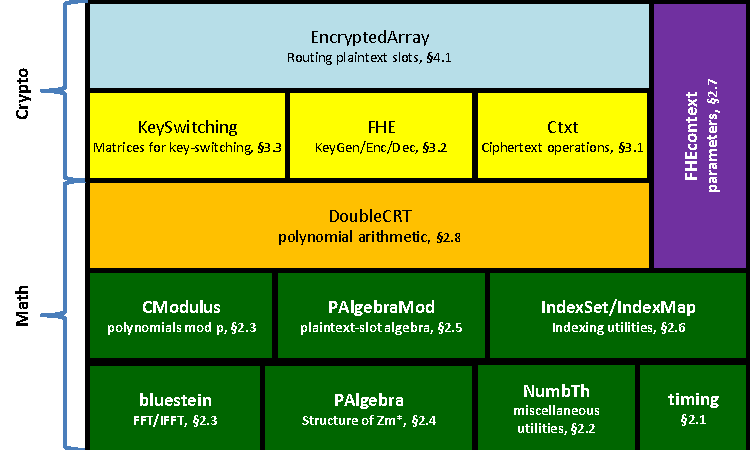
\includegraphics{HElibrary.pdf}}
\else
\vspace{2in}
\fi
\caption{A block diagram of the Homomorphic-Encryption library}
\label{fig:blocks}
\end{figure}

%%%%%%%%%%%%%%%%%%%%%%%%%%%%%%%%%%%%%%%%%%%%%%%%%%%%%%%%%%%%%%%%%%%%%%
\section{The Math Layers} \label{sec:math}
%%%%%%%%%%%%%%%%%%%%%%%%%%%%%%%%%%%%%%%%%%%%%%%%%%%%%%%%%%%%%%%%%%%%%%
\subsection{The \texttt{timing} module}\label{timing}
This module contains some utility functions for measuring the time
that various methods take to execute. To use it, we insert the macro
\texttt{FHE\_TIMER\_START} at the beginning of the method(s) that we
want to time and \texttt{FHE\_TIMER\_STOP} at the end, then the main
program needs to call the function \texttt{setTimersOn()} to activate
the timers and \texttt{setTimersOff()} to pause them. 
We can have at most one timer per method/function, and the timer
is called by the same name as the function itself (using the
built-in macro \texttt{\_\_func\_\_}). To obtain the value
of a given timer (in seconds), the application can use the function
\texttt{double getTime4func(const char *fncName)}, and the function
\texttt{printAllTimers()} prints the values of all timers to the
standard output.

%%%%%%%%%%%%%%%%%%%%%%%%%%%%%%%%%%%%%%%%%%%%%%%%%%%%%%%%%%%%%%%%%%%%%%
\subsection{{\NumbTh}: Miscellaneous Utilities}
\label{sec:numbTh}
This module started out as an implementation of some number-theoretic
algorithms (hence the name), but since then it grew to include many
different little utility functions. For example, CRT-reconstruction
of polynomials in coefficient representation, conversion functions
between different types, procedures to sample at random from various
distributions, etc.

%%%%%%%%%%%%%%%%%%%%%%%%%%%%%%%%%%%%%%%%%%%%%%%%%%%%%%%%%%%%%%%%%%%%%%
\subsection{{\bluestein} and {\Cmodulus}: Polynomials in FFT Representation}
\label{sec:bluestein} \label{sec:Cmodulus}
The {\bluestein} module implements a non-power-of-two FFT over a prime
field $\Z_p$, using the Bluestein FFT algorithm \cite{bluestein}. We
use modulo-$p$ polynomials to encode the FFTs inputs and outputs.
Specifically this module builds on Shoup's NTL library \cite{NTL},
and contains both a bigint version with types \texttt{ZZ\_p} and
\texttt{ZZ\_pX}, and a smallint version with types \texttt{zz\_p}
and \texttt{zz\_pX}.
We have the following functions:
\begin{verbatim}
void BluesteinFFT(ZZ_pX& x, long n,
                  const ZZ_p& root, ZZ_pX& powers, 
                  Vec<mulmod_precon_t>& powers_aux, 
                  FFTRep& Rb, fftrep_aux& Rb_aux, FFTRep& Ra);

void BluesteinFFT(zz_pX& x, long n,
                  const zz_p& root, zz_pX& powers, 
                  Vec<mulmod_precon_t>& powers_aux, 
                  fftRep& Rb, fftrep_aux& Rb_aux, fftRep& Ra);
\end{verbatim}
These functions compute length-$n$ FFT of the coefficient-vector of
\texttt{x} and put the result back in \texttt{x}. If the degree of
\texttt{x} is less than $n$ then it treats the top coefficients as~0,
and if the degree is more than~$n$ then the extra coefficients are
ignored. Similarly, if the top entries in the result \texttt{x} are
zeros then \texttt{x} will have degree smaller than~$n$. The argument
\texttt{root} needs to be a \emph{$2n$-th root of unity} in $\Z_p$.
%
The inverse-FFT is obtained just by calling
\texttt{BluesteinFFT(...,root}$^{-1}$\texttt{,...)}, but this
procedure is \emph{NOT SCALED}. Hence calling
\texttt{BluesteinFFT(x,a,n,root,...)} and then 
\texttt{BluesteinFFT(b,x,n,root}$^{-1}$\texttt{,...)} will result
in having $\mathtt{b}=n \times \mathtt{a}$.

In addition to the size-$n$ FFT of a which is returned in \texttt{x},
this procedure also returns the powers of \texttt{root} in the
\texttt{powers} argument,
$\mathtt{powers} = \big(1, \mathtt{root}, \mathtt{root}^4, \mathtt{root}^9, 
\ldots, \mathtt{root}^{(n-1)^2}\big).$
In the \texttt{Rb} argument it returns the size-$N$ FFT representation
of the negative powers, for some $N \ge 2n-1$, $N$ a power of two:
\begin{eqnarray*}
\mathbf{Rb} &=& FFT_N\big(0,\ldots,0,
  \mathtt{root}^{-(n-1)^2},\ldots,\mathtt{root}^{-4},\mathtt{root}^{-1},
  1, \mathtt{root}^{-1}, \mathtt{root}^{-4},\ldots,\mathtt{root}^{-(n-1)^2}
  0,\ldots,0\big).
\end{eqnarray*}
On subsequent calls with the same \texttt{powers} and \texttt{Rb},
these arrays are not computed again but taken from the pre-computed
arguments. If the \texttt{powers} and \texttt{Rb} arguments are
initialized, then it is assumed that they were computed correctly from
\texttt{root}. The behavior is undefined when calling with initialized
\texttt{powers} and \texttt{Rb} but a different \texttt{root}.
(In particular, to compute the inverse-FFT using $\mathtt{root}^{-1}$,
one must provide different \texttt{powers} and \texttt{Rb} arguments
than those that were given when computing in the forward direction
using \texttt{root}.)
%To reset these arguments between calls with different \texttt{root}
%values, use clear(powers); Rb.SetSize(0);

The parameters \texttt{powers\_aux} and \texttt{Rb\_aux} are just used to store 
precomputed results depending on \texttt{powers} and \text{Rb}, respectively, 
from one call to the next: the caller should make sure that 
the same objects are consistently passed. 
The parameter \texttt{Ra} is just used for temporary storage,
to minimize memory allocations.


\paragraph{The classes \texttt{Cmodulus} and \texttt{CModulus}.}
These classes provide an interface layer for the FFT routines above,
relative to a single prime (where \texttt{Cmodulus} is used for
smallint primes and \texttt{CModulus} for bigint primes). They keep
the NTL ``current modulus'' structure for that prime, as well as the
auxiliary structures
\texttt{powers}, \texttt{Rb}, \texttt{powers\_aux},
\texttt{Rb\_aux}, and \texttt{Ra} arrays for FFT and inverse-FFT under
that prime. They are constructed with the constructors

\smallskip
\texttt{Cmodulus(const PAlgebra\& ZmStar, const long\& q, const long\& root);}

\texttt{CModulus(const PAlgebra\& ZmStar, const ZZ\& q, const ZZ\& root);}

\smallskip\noindent
where \texttt{ZmStar} described the structure of $\Z_m^*$ (see
\secref{PAlgebra}), \texttt{q} is the prime modulus and \texttt{root}
is a primitive $2m-$'th root of unity modulo~$q$. (If the constructor
is called with $\mathtt{root}=0$ then it computes a $2m$-th root of
unity by itself.) Once an object of one of these classes is
constructed, it provides an FFT interfaces via

\smallskip
\texttt{void Cmodulus::FFT(vec\_long\& y, const ZZX\& x) const;~ // y = FFT(x)}

\texttt{void Cmodulus::iFFT(ZZX\& x, const vec\_long\& y) const; // x = FFT$^{-1}$(y)}

\smallskip\noindent
(And similarly for \texttt{CModulus} using \texttt{vec\_ZZ} instead of
\texttt{vec\_long}). These method are inverses of each other. 

%%%%%%%%%%%%%%%%%%%%%%%%%%%%%%%%%%%%%%%%%%%%%%%%%%%%%%%%%%%%%%%%%%%%%%
\subsection{{\PAlgebra}: The Structure of $\Z_m^*$ and $\Z_m^*/\grp{2}$}
\label{sec:PAlgebra}
The class {\PAlgebra} is the base class containing the structure
of $\Z_m^*$, as well as the quotient group $\Z_m^*/\grp{2}$. We
represent $\Z_m^*$ as $\Z_m^*= \grp{2} \times \grp{g_1,g_2,\ldots}
\times\grp{h_1,h_2,\ldots}$, where each $g_i$ has the same order
in $\Z_m^*$ as in $\Z_m^*/\grp{2,g_1,\ldots,g_{i-1}}$, and the
$h_i$'s generate the group $\Z_m^*/\grp{2,g_1,g_2,\ldots}$ (and they do
not have the same order in $\Z_m^*$ as in $\Z_m^*/\grp{2,g_1,\ldots}$).

We compute this representation in a manner similar (but not identical)
to the proof of the fundamental theorem of finitely generated abelian
groups. Namely we keep the elements in equivalence classes of the
``quotient group so far'', and each class has a representative element
(called a pivot), which in our case we just choose to be the smallest
element in the class. Initially each element is in its own class.
At every step, we choose the highest order element~$g$ in the current
quotient group and add it as a new generator, then unify classes if
their members are a factor of~$g$ from each other, repeating this
process until no further unification is possible.
Since we are interested in the quotient group $\Z_m^*/\grp{2}$, we
always choose~2 as the first generator.

One twist in this routine is that initially we only choose an element
as a new generator if its order in the current quotient group is the
same as in the original group~$\Z_m^*$. Only after no such elements
are available, do we begin to use generators that do not have the
same order as in~$\Z_m^*$.

Once we chose all the generators (and for each generator we compute
its order in the quotient group where it was chosen), we compute a
set of ``slot representatives'' as follows: Putting all the $g_i$'s
and $h_i$'s in one list, let us denote the generators of $\Z_m^*/
\grp{2}$ by $\{f_1,f_2,\ldots,f_n\}$, and let $\ord(f_i)$ be the
order of $f_i$ in the quotient group at the time that it was added
to the list of generators. The the slot-index representative set is
\[
T ~\eqdef~ \left\{ \prod_{i=1}^n f_i^{e_i} \bmod m ~:~
   ~\forall i, e_i \in \{0,1,\ldots,\ord(f_i)-1\} \right\}.
\]
Clearly, we have $T\subset\Z_m^*$, and moreover $T$ contains exactly
one representative from each equivalence class of $\Z_m^*/\grp{2}$.
Recall that we use these representatives in our encoding of plaintext
slots, where a polynomial $a\in\A_2$ is viewed as encoding the vector
of $\F_{2^d}$ elements $\big(a(\rho^t)\in\F_{2^d}~:~t\in T\big)$,
where $\rho$ is some fixed primitive $m$-th root of unity in
$\F_{2^d}$.

In addition to defining the sets of generators and representatives,
the class {\PAlgebra} also provides translation methods between
representations, specifically:
\begin{description}
\item[\texttt{int ith\_rep(unsigned i) const;}]\ \\
  Returns~$t_i$, i.e., the $i$'th representative from~$T$.
\item[\texttt{int indexOfRep(unsigned t) const;}]\ \\
  Returns the index~$i$ such that \texttt{ith\_rep}$(i)=t$.

\item[]\hspace{-0.5em}\texttt{int exponentiate(const vector<unsigned>\& exps, \newline 
              bool onlySameOrd=false) const;}\ \\
  Takes a vector of exponents, $(e_1,\ldots,e_n)$ and returns
  $t = \prod_{i=1}^n f_i^{e_i} \in T$.

\item[\texttt{const int* dLog(unsigned t) const;}]\ \\
  On input some $t\in T$, returns the discrete-logarithm of~$t$ with
  the $f_i$'s are bases. Namely, a vector \texttt{exps}$=(e_1,\ldots,
  e_n)$ such that \texttt{exponentiate(exps)}$=t$, and moreover
  $0\le e_i\le\ord(f_i)$ for all~$i$.
\end{description}

In fact, our implementation is slightly more general.
The special generator $2$ map be replaced with an arbitrary prime $p$.
The constructor for the class {\PAlgebra} is:
\begin{verbatim}
   PAlgebra(unsigned m, unsigned p = 2); 
\end{verbatim}
Thus, a {\PAlgebra} object is completely determined by $m$ and $p$,
where $p$ defaults to $p = 2$.



%%%%%%%%%%%%%%%%%%%%%%%%%%%%%%%%%%%%%%%%%%%%%%%%%%%%%%%%%%%%%%%%%%%%%%
\subsection{{\PAlgebraMod}: Plaintext Slots}
\label{sec:PAlgebraTwo}\label{sec:PAlgebraTwoR}
This class implements the structure of the plaintext spaces,
which is of the form $\A_{p^r} = \A/p^r \A$,
for a small value of $r$.
Recall that $\A = \Z[X]/(\Phi_m(X))$
and $\A_{p^r} = \A/(p^r) = \Z[X]/(\Phi_m(X), p^r)$.
Typically, $r = 1$ for ordinary homomorphic computation,
while we expect to use $r > 1$ for bootstrapping,
as described in
\cite{GHS12b}. 
Also note that while, typically, $p=2$ (the default value for $p$
when constructing a {\PAlgebra} object), an arbitrary prime $p$
is allowed.


For the case $r=1$, the plaintext slots are determined by the
factorization of $\Phi_m(X)$ modulo $p$ into $\ell$ degree-$d$
polynomials. 
Once we have this factorization, $\Phi_m(X)=\prod_j
F_j(X)\pmod{p}$, we choose an arbitrary factor as the ``first factor'',
denote it $F_1(X)$, and this corresponds to the first input slot
(whose representative is $1\in T$).% 
\footnote{
In the current implementation, a natural lexicographic order
is imposed on polynomials modulo $p$, and the smallest
such factor with respect to this order is chosen as $F_1$.
This ensures interoperability across different platforms.
}
With each representative $t\in T$
we then associate the factor $GCD(F_1(X^t),\Phi_m(X))$, with
polynomial-GCD computed modulo $p$. 
Note that fixing a representation of the field $\K=\Z_p[X]/(F_1(X))
\cong \F_{p^d}$ and letting $\rho$ be a root of~$F_1$ in~$\K$, we get
that the factor associated with the representative~$t$ is the minimal
polynomial of $\rho^{1/t}$. Yet another way of saying the same thing,
if the roots of $F_1$ in~$\K$ are \[\rho,\rho^p,\rho^{p^2},\ldots,
\rho^{p^{d-1}},\] then the roots of the factor associated to~$t$ are
\[\rho^{1/t},\rho^{p/t},\rho^{p^2/t},\ldots,\rho^{p^{d-1}/t},\] where
the arithmetic in the exponent is modulo~$m$.

For the case $r > 1$, we start with a factorization
of $\Phi_m(X)$ modulo $p$ as above, and then use
Hensel lifting to obtain a factorization 
of $\Phi_m(X)$ modulo $p^r$.
Note that even in the case where $r > 1$ and we set 
$\K = \Z_{p^r}[X]/(F_1)$, the very same correspondence
among roots as noted in the previous paragraph still
holds in this setting.
Among other things, this correspondence guarantees
that the various plaintext slot rings $\Z_{p^r}[X]/(F_i)$
are all isomorphic.
%\victorsays{This sketches the justification of the isomorphism claim.
%It doesn't seem to be a particularly ``standard'' fact.
%}

After computing the factors of $\Phi_m(X)$ modulo $p^r$ and the
correspondence between these factors and the representatives from~$T$,
the class {\PAlgebraMod} provides encoding/decoding methods to pack
elements in polynomials and unpack them back. 
This is really the main functionality provided by this class,
and we shall proceed to describe the interface in some detail.


An object \var{alMod} of type {\PAlgebraMod} holds the integer~$r$,
along with a {\PAlgebra} object \var{zMStar}, which determines $p$
and $m$. The object \var{alMod} also provides
support for encoding and decoding plaintext slots, with respect
to a specified plaintext slot subring as determined by a polynomial
$G(X)$. If $r = 1$, then $G(X)$ may be any irreducible polynomial
over $\Z_p$ whose degree divides $d$. (For example, for homomorphic
AES we can use and $d$ divisible by~8, and $G$ will be the AES
polynomial $G(X)=X^8 + X^4 + X^3 + X + 1$.)

For $r > 1$, our current implementation is more restrictive,
requiring that either $\deg G(X) = 1$ or $G(X) = F_1$.
With these constraints, we are ensured that the $\Z_{p^r}[X]/(G)$
corresponds to a subring of each of the plaintext slot rings 
$\Z_{p^r}[X]/(F_i)$ via an efficiently computable 
$\Z_{p^r}$-algebra isomorphism.

The {\PAlgebraMod} object \var{alMod} stores various tables
of objects in the polynomial ring $\Z_{p^r}[X]$.  To do this most 
efficiently, if $p = 2$ and $r = 1$, then these polynomials
are represented as NTL objects of type \class{GF2X}, 
and otherwise of type \class{zz_pX}. 
Thus, the types of these objects are not determined until run time.
As such, we use a class hierarchy, as follows.
\begin{itemize}
\item
\class{PAlgebraModBase} is a virtual base class

\item
\class{PAlegbraModDerived<type>} is a derived template class, where
\class{type} is either \class{PA_GF2} or \class{PA_zz_p}.

These latter two classes define various types representing
polynomials, vectors, and other objects related to the choice of
underlying representation, all defined via {\tt typedef}'s.

\item
The class \class{PAlgebraMod} itself is a simple 
wrapper around a smart pointer to a
\class{PAlgebraModBase} object: copying a \class{PAlgebraMod} 
object results is
a ``deep copy'' of the underlying object of the derived class.
\end{itemize}

The slot encoding/decoding operations 
cannot be performed directly using a \class{PAlgebraMod}
object, but rather, they must be performed using objects
of the derived class.
So, given an object of type \class{PAlgebraMod},
which contains a pointer to an object of type
\class{PAlgebraModBase}, one must first 
 ``downcast'' this pointer to a pointer of type
\class{PAlgebraModDerived<type>}.
For convenience, the class \class{PAlgebraMod}
provides a special ``downcast'' method to simplify the notation.

As discussed above, slot encoding and decoding is done
with respect to a slot subring defined by a polynomial
$G \in \Z_{p^r}[X]$.
A call to the following method of \class{PAlgebraModDerived<type>}
will precompute relevant data determined by $G$:
\begin{verbatim}
  void mapToSlots(MappingData<type>& mappingData, const RX& G) const;
\end{verbatim}
The precomputed data is stored in the parameter \class{mappingData},
which is a template type, parameterized in the same
way as \class{PAlgebraModDerived}.
Also, \class{RX} is a \class{typedef}
that is defined as either \class{GF2X} or \class{zz_pX},
depending on the class parameter \class{type}.

A call to the the following method of \class{PAlegbraModDerived<type>}
will create a plaintext (which is a polynomial modulo $p^r$) 
by embedding a vector of polynomials (modulo $G$) into the corresponding
slots:
\begin{verbatim}
  void embedInSlots(RX& H, const vector<RX>& alphas, 
                    const MappingData<type>& mappingData) const;
\end{verbatim}
Here, \class{mappingData} holds the precomputed data obtained
from \class{mapToSlots}, \class{alphas} is the
vector of slot values, and the resulting plaintext
is stored in \class{H}.

The following method of \class{PAlegbraModDerived<type>} does the
same thing, but embeds the same value \class{alpha} in each slot:
\begin{verbatim}
  void embedInAllSlots(RX& H, const RX& alpha, 
                       const MappingData<type>& mappingData) const;
\end{verbatim}

The following method of \class{PAlegbraModDerived<type>} reverses
the process, unpacking the slots of a given plaintext \class{ptxt}
into a vector \class{alphas}:
\begin{verbatim}
  void decodePlaintext(vector<RX>& alphas, const RX& ptxt,
		       const MappingData<type>& mappingData) const;
\end{verbatim}

Usage of the \texttt{PAlgebraMod} classes is similar to the
higher-level \texttt{EncryptedArray} classes, as illustrated in
\secref{usingEncryptedArrays}.

\subsubsection*{Other functionality}
Besides slot encoding/decoding, the class \class{PAlgebraMod} provides
some other functionality as well.

First, a  \class{PAlgebraMod} object stores some ``mask tables''
which is used by the class \class{EncryptedArray} --- these
tables help facilitate rotating the slots of encrypted data.

Second, a \class{PAlgebraMod} object may be used to
to calculate the ``linearized polynomial'' associated
to a $\Z_{p^r}$-linear map over $\Z_{p^r}[X]/(G)$.
The interface here is similar to the slot encoding/decoding
interface, in that the operations are performed using a
\class{PAlgebraModDerived} object and a \class{MappingData}
object defined by $G$.
The following \class{PAlgebraModDerived}-method
\begin{verbatim}
  void buildLinPolyCoeffs(vector<RX>& C, const vector<RX>& L,
                          const MappingData<type>& mappingData) const;
\end{verbatim}
will compute the coefficient vector $C$ corresponding to 
a linear map $M$ described using $L$ by its action on the
power basis for $\Z_{p^r}[X]/(G)$;
that is,  $M(x^j \bmod G) = (L[j] \bmod G)$,
  for $j = 0 \ldots d-1$.  
The result is a coefficient vector $C$ for the linearized
polynomial representing $M$:   for $h \in Z_{p^r}[X]$ of degree $< d$,  
$M(h(X) \bmod G) = \sum_{i=0}^{d-1} (C[j] \mod G) \cdot (h(X^{p^j}) \mod G)$.

Note that in the case where $r = 1$, such linearized polynomials
are guaranteed to exist, according to the standard theory 
of finite fields. One can also show that such linearized polynomials
exist also in the case $r > 1$, since $C$ is 
the solution to a linear system of equations,
and so it exists and be computed by Hensel lifting
from a solution modulo $p$.
(We remark that the method \class{buildLinPolyCoeffs} is used
by \class{EncryptedArray} class, that that class also provides
a higher-level interface.)


%%%%%%%%%%%%%%%%%%%%%%%%%%%%%%%%%%%%%%%%%%%%%%%%%%%%%%%%%%%%%%%%%%%%%%
\subsection{{\IndexSet} and {\IndexMap}: Sets and Indexes}
\label{sec:IndexSet} \label{sec:IndexMap}
In our implementation, all the polynomials are represented in
double-CRT format, relative to some subset of the small primes in
our list (cf. \secref{dcrt}). The subset itself keeps changing
throughout the computation, and so we can have the same polynomial
represented at one point relative to many primes, then a small
number of primes, then many primes again, etc. (For example see the
implementation of key-switching in \secref{keySwitching}.) To provide
flexibility with these transformations, the {\IndexSet} class
implements an arbitrary subset of nonnegative integers, and the {\IndexMap}
class implements a collection of data items that are indexed by such
a subset.

%---------------------------------------------------------------------
\subsubsection{The {\IndexSet} class}
The {\IndexSet} class implements all the standard interfaces of the
abstract data-type of a set, along with just a few extra interfaces
that are specialized to sets of \emph{nonnegative integers}. It uses the standard
C++ container \texttt{vector<bool>} to keep the actual set, and
provides the following methods:
\begin{description}
\item[Constructors.] The constructors \texttt{IndexSet()},
\texttt{IndexSet(long j)}, and \texttt{IndexSet(long low, long high)},
initialize an empty set, a singleton, and an interval,
respectively.

\item[Empty sets and cardinality.]
The static method {\IndexSet}\texttt{::emptySet()}
provides a read-only access to an empty set, and the method
\texttt{s.clear()} removes all the elements in \texttt{s}, which
is equivalent to \texttt{s}$=${\IndexSet}\texttt{::emptySet()}.

The method \texttt{s.card()} returns the number of elements in 
\texttt{s}.

\item[Traversing a set.] The methods \texttt{s.first()} and
\texttt{s.last()} return the smallest and largest element in the
set, respectively. For an empty set \texttt{s}, \texttt{s.first()}
returns 0 and \texttt{s.last()} returns~$-1$.

The method \texttt{s.next($j$)} return the next element after~$j$,
if any; otherwise $j+1$. Similarly \texttt{s.prev($j$)} return the
previous element before~$j$, if any; otherwise $j-1$. With these
methods, we can iterate through a set \texttt{s} using one of:\\
\mbox{~~~~}\texttt{for (long i = s.first(); i <= s.last(); i = s.next(i)) ...}\\
\mbox{~~~~}\texttt{for (long i = s.last(); i >= s.first(); i = s.prev(i)) ...}

\item[Comparison and membership methods.] 
\texttt{operator==} and \texttt{operator!=} are provided to
test for equality, whereas \texttt{s1.disjointFrom(s2)} and its
synonym \texttt{disjoint(s1,s2)} test if the two sets are disjoint.
Also,
\texttt{s.contains(j)} returns \texttt{true} if \texttt{s} contains
the element~$j$, \texttt{s.contains(other)} returns \texttt{true}
if \texttt{s} is a superset of \texttt{other}. For convenience, the
operators \texttt{<=}, \texttt{<}, \texttt{>=} and \texttt{>} are
also provided for testing the subset relation between sets.

\item[Set operations.] 
The method \texttt{s.insert(j)} inserts the integer~$j$ if it is not
in \texttt{s}, and \texttt{s.remove(j)} removes it if it is there.

Similarly \texttt{s1.insert(s2)} returns in \texttt{s1} the union of
the two sets, and \texttt{s1.remove(s2)} returns in \texttt{s1} the
set difference $\mathtt{s1\setminus s2}$. Also, \texttt{s1.retain(s2)}
returns in \texttt{s1} the intersection of the two sets.
For convenience we also provide the operators \texttt{s1|s2} (union),
\texttt{s1\&s2} (intersection), \texttt{s1}\texttt{\^}\texttt{s2}
(symmetric difference, aka xor), and \texttt{s1/s2} (set difference). 
\end{description}

%---------------------------------------------------------------------
\subsubsection{The {\IndexMap} class}
The class template {\IndexMap}\texttt{<T>} implements a map of elements
of type \texttt{T}, indexed by a dynamic {\IndexSet}.  Additionally, it
allows new elements of the map to be initialized in a flexible manner,
by providing an initialization function which is called whenever a new
element (indexed by a new index~$j$) is added to the map. 

Specifically, we have a helper class template \texttt{IndexMapInit<T>}
that stores a pointer to an initialization function, and possibly also
other parameters that the initialization function needs. We 
then provide a constructor 
\begin{quote}
{\IndexMap}\texttt{(IndexMapInit<T>*
initObject=nullptr)} 
\end{quote}
that associates the given initialization object
with the new {\IndexMap} object.
Thereafter, when a new index~$j$ is added to the index set, an object
\texttt{t} of type \texttt{T} is created using the default constructor
for \texttt{T}, after which the function \texttt{initObject->init(t)}
is called.

In our library, we use an {\IndexMap} to store the rows of the matrix
of a Double-CRT object. For these objects we have an initialization
object that stores the value of $\phi(m)$, and the initialization
function, which is called whenever we add a new row, ensures that all
the rows have length exactly~$\phi(m)$.

After initialization, an {\IndexMap} object provides the operator
\texttt{map[i]} to access the type-\texttt{T} object indexed by~$i$
(if $i$ currently belongs to the {\IndexSet}), as well as the methods
\texttt{map.insert(i)} and \texttt{map.remove(i)} to insert or delete
a single data item indexed by~$i$, and also \texttt{map.insert(s)} and
\texttt{map.remove(s)}  to insert or delete a collection of data items
indexed by the {\IndexSet} \texttt{s}.

%%%%%%%%%%%%%%%%%%%%%%%%%%%%%%%%%%%%%%%%%%%%%%%%%%%%%%%%%%%%%%%%%%%%%%
\subsection{{\FHEcontext}: Keeping the parameters}\label{sec:FHEcontext}
Objects in higher layers of our library are defined
relative to some parameters, such as the integer parameter~$m$ (that
defines the groups $\Z_m^*$ and $\Z_m^*/\grp{p}$ and the ring $\A=
\Z[X]/\Phi_m(X)$) and the sequence of small primes that determine our
modulus-chain. To allow convenient access to these parameters, we
define the class {\FHEcontext} that keeps them all and provides
access methods and some utility functions.

One thing that's included in {\FHEcontext} is a vector of {\Cmodulus}
objects, holding the small primes that define our modulus chain:
\begin{verbatim}
  vector<Cmodulus> moduli;  // Cmodulus objects for the different primes
\end{verbatim}

We provide access to the {\Cmodulus} objects via
\texttt{context.ithModulus(i)} (that returns a reference of type
\texttt{const Cmodulus\&}), and to the small primes themselves via
\texttt{context.ithPrime(i)} (that returns a \texttt{long}).
The {\FHEcontext} includes also the various algebraic structures for
plaintext arithmetic, specifically we have the three data members:

\smallskip\begin{tabular}{ll}
\texttt{PAlgebra zMstar;}
   & \texttt{// The structure of} $\Z_m^*/\langle p \rangle$ \\
\texttt{PAlgebraMod alMod;}
   & \texttt{// The structure of} $\Z[X]/(\Phi_m(X),p^r)$
\end{tabular}

\medskip
In addition to the above, the {\FHEcontext} contains a few
{\IndexSet} objects, describing various partitions of the index-set in
the vector of moduli. These partitions are used when generating the
key-switching matrices in the public key, and when using them to
actually perform key-switching on ciphertexts.

One such partition is ``ciphertext'' vs. ``special'' primes:
Freshly encrypted ciphertexts are encrypted relative to a subset of
the small primes, called the \emph{ciphertext primes}. All other
primes are only used during key-switching, these are called the
\emph{special primes}. The ciphertext primes, in turn, are sometimes
partitioned further into a number of ``digits'', corresponding to the
columns in our key-switching matrices. (See the explanation of this
partition in \secref{keySwitching}.) These subsets are stored
in the following data members:
\begin{verbatim}
  IndexSet ctxtPrimes;     // the ciphertext primes
  IndexSet specialPrimes;  // the "special" primes
  vector<IndexSet> digits; // digits of ctxt/columns of key-switching matrix
\end{verbatim}

The {\FHEcontext} class provides also some convenience functions for
computing the product of a subset of small primes, as well as the
``size'' of that product (i.e., its logarithm), via the methods:

\begin{verbatim}
  ZZ productOfPrimes(const IndexSet& s) const;
  void productOfPrimes(ZZ& p, const IndexSet& s) const;

  double logOfPrime(unsigned i) const;   // = log(ithPrime(i))
  double logOfProduct(const IndexSet& s) const;
\end{verbatim}

Finally, the {\FHEcontext} module includes some utility functions for
choosing parameters and adding moduli to the chain.
The method \texttt{addPrime(long p, bool isSpecial)} adds a single
prime~$p$ (either ``special'' or not), after checking that~$p$ has
$2m$'th roots of unity and it is not already in the list. Then we
have three higher-level functions:

\begin{description}
\item[\texttt{double AddPrimesBySize(FHEcontext\& c, double size, bool special=false);}]\ \\
Adds to the chain primes whose product is at least exp(\texttt{size}), returns the natural logarithm of the product of all added primes.

\item[\texttt{double AddPrimesByNumber(FHEcontext\& c, long n, long atLeast=1, bool special=false);}]
Adds $n$ primes to the chain, all at least as large as the \texttt{atLeast} argument, returns the natural logarithm of the product of all added primes.

\item[\texttt{void buildModChain(FHEcontext\& c, long d, long t=3);}]\ \\
Build modulus chain for a circuit of depth $d$, using $t$ digits in key-switching. This function puts~$d$ ciphertext primes in the \texttt{moduli} vector, and then as many ``special'' primes as needed to mod-switch fresh ciphertexts
(see \secref{keySwitching}).
\end{description}
We also have a helper function that uses some pre-computed table to
help select the values for the parameter~$m$ (defining the $m$'th
cyclotomic ring):

\smallskip
\texttt{long FindM(long k, long L, long c, long p, long d, long s, long chosen\_m, bool verbose=false);}

\smallskip\noindent
In this method, $\mathtt{k}$ is the security parameter, $\mathtt{L}$ is the number of ciphertext-primes that we want to support, $\mathtt{c}$ is the number of columns in our key-switching matrices. The arguments~$\mathtt{p,d}$ determine the plaintext space $\F_{p^d}$, the argument $\mathtt{s}$ bounds from below the number of plaintext slots that we want to support, and \texttt{chosen\_m} gives the ability to specify a particular $m$ parameter and test if it satisfies all our constraints.

%%%%%%%%%%%%%%%%%%%%%%%%%%%%%%%%%%%%%%%%%%%%%%%%%%%%%%%%%%%%%%%%%%%%%%
\subsection{{\DoubleCRT}: Efficient Polynomial Arithmetic}
\label{sec:DoubleCRT}
The heart of our library is the {\DoubleCRT} class that manipulates
polynomials in Double-CRT representation. A {\DoubleCRT} object is
tied to a specific {\FHEcontext}, and at any given time it is defined
relative to a subset of small primes from our list, $S\subseteq
[0,\ldots,\mathtt{context.moduli.size()}-1]$. Denoting the product of
these small primes by $q=\prod_{i\in S} p_i$, a {\DoubleCRT} object
represents a polynomial $a\in\A_q$ by a matrix with $\phi(m)$ columns
and one row for each small prime $p_i$ (with $i\in S$). The $i$'th
row contains the FFT representation of~$a$ modulo~$p_i$, i.e., the
evaluations $\{[a(\zeta_i^{~j})]_{p_i}~:~j\in\Z_m^*\}$, where
$\zeta_i$ is some primitive $m$-th root of unity modulo~$p_i$.

Although the {\FHEcontext} must remain fixed throughout, the set~$S$
of primes can change dynamically, and so the matrix can lose some rows
and add other ones as we go. We thus keep these rows in a dynamic
{\IndexMap} data member, and the current set of indexes~$S$ is
available via the method \texttt{getIndexSet()}. We provide the
following methods for changing the set of primes:
\begin{description}
\item[\texttt{void addPrimes(const IndexSet\& s);}]\ \\
Expand the index set by \texttt{s}. It is assumed that \texttt{s} is
disjoint from the current index set. This is an expensive operation,
as it needs to convert to coefficient representation and back, in
order to determine the values in the added rows.
  
\item[\texttt{double addPrimesAndScale(const IndexSet\& S);}]\ \\
Expand the index set by \texttt{S}, and multiply by $q_{\mathrm{diff}}
=\prod_{i \in S}p_i$. The set \texttt{S} is assumed to be disjoint
from the current index set. Returns $\log(q_{\mathrm{diff}})$. This
operation is typically much faster than \texttt{addPrimes}, since we
can fill the added rows with zeros.

\item[\texttt{void removePrimes(const IndexSet\& s);}]\ \\
Remove the primes $p_i$ with $i\in\mathtt{s}$ from the current
index set.

\item[\texttt{void scaleDownToSet(const IndexSet\& s, long ptxtSpace);}]\ \\
This is a modulus-switching operation. Let $\Delta$ be the set of
primes that are removed, $\Delta=\mathtt{getIndexSet()\setminus s}$,
and  $q_{\mathrm{diff}}=\prod_{i \in \Delta}p_i$. This operation
removes the primes $p_i, i\in\Delta$, scales down the polynomial by a
factor of $q_{\mathrm{diff}}$ (hence getting a fractional polynomial),
and rounds to an integer so as to keep $a \bmod\mathtt{ptxtSpace}$
unchanged.
\end{description}

We provide some conversion routines to convert polynomials from
coefficient-representation (NTL's \texttt{ZZX} format) to {\DoubleCRT}
and back, using the constructor 

\smallskip
\texttt{DoubleCRT(const ZZX\&, const FHEcontext\&, const IndexSet\&);}

\smallskip\noindent
and the conversion function \texttt{ZZX to\_ZZX(const DoubleCRT\&)}.
%We also provide translation routines between {\SingleCRT} and {\DoubleCRT}.

We support the usual set of arithmetic operations on {\DoubleCRT}
objects (e.g., addition, multiplication, etc.), always working in
$\A_q$ for some modulus~$q$.  We only implemented the ``destructive''
two-argument version of these operations, where one of the input
arguments is modified to return the result.  These arithmetic
operations can only be applied to {\DoubleCRT} objects relative to the
same {\FHEcontext}, else an error is raised.

The
{\DoubleCRT} class supports operations between objects with different
{\IndexSet}'s, offering two options to resolve the differences: our
arithmetic operations take a boolean flag \texttt{matchIndexSets};
when the flag is set to \emph{true} (which is the default), the
index-set of the result is the union of the index-sets of the two
arguments. When \texttt{matchIndexSets}$=$\emph{false} then the
index-set of the result is the same as the index-set of \texttt{*this},
i.e., the argument that will contain the result when the operation
ends. The option \texttt{matchIndexSets}$=$\emph{true} is slower,
since it may require adding primes to the two arguments. Below is
a list of the arithmetic routines that we implemented:

\begin{verbatim}
  DoubleCRT& Negate(const DoubleCRT& other); // *this = -other
  DoubleCRT& Negate();                       // *this = -*this;

  DoubleCRT& operator+=(const DoubleCRT &other); // Addition
  DoubleCRT& operator+=(const ZZX &poly); // expensive
  DoubleCRT& operator+=(const ZZ &num);
  DoubleCRT& operator+=(long num);

  DoubleCRT& operator-=(const DoubleCRT &other); // Subtraction
  DoubleCRT& operator-=(const ZZX &poly); // expensive
  DoubleCRT& operator-=(const ZZ &num);
  DoubleCRT& operator-=(long num);

  // These are the prefix versions, ++dcrt and --dcrt. 
  DoubleCRT& operator++();
  DoubleCRT& operator--();

  // Postfix versions (return type is void, it is offered just for style)
  void operator++(int);
  void operator--(int);

  DoubleCRT& operator*=(const DoubleCRT &other); // Multiplication
  DoubleCRT& operator*=(const ZZX &poly); // expensive
  DoubleCRT& operator*=(const ZZ &num);
  DoubleCRT& operator*=(long num);

  // Procedural equivalents, providing also the matchIndexSets flag

  void Add(const DoubleCRT &other, bool matchIndexSets=true);
  void Sub(const DoubleCRT &other, bool matchIndexSets=true);
  void Mul(const DoubleCRT &other, bool matchIndexSets=true);

  DoubleCRT& operator/=(const ZZ &num);  // Division by constant
  DoubleCRT& operator/=(long num);

  void Exp(long k);    // Small-exponent polynomial exponentiation

  // Automorphism F(X) --> F(X^k)  (with gcd(k,m)==1)
  void automorph(long k);
  DoubleCRT& operator>>=(long k);
\end{verbatim}

\noindent
We also provide methods for choosing at random polynomials in
{\DoubleCRT} format, as follows:
%\shaisays{Except the first of these, all the others use
%\texttt{lrand48}, we should probably switch to using the NTL PRG
%instead.}

\begin{description}
\item[\texttt{void randomize(const ZZ* seed=nullptr);}]\ \\
Fills each row~$i\in\mathtt{getIndexSet()}$ with random integers 
modulo~$p_i$. This procedure uses the NTL PRG, setting the seed
to the \texttt{seed} argument if it is non-nullptr, and using the
current PRG state of NTL otherwise.

\item[\texttt{void sampleSmall();}]\ \\
Draws a random polynomial in coefficient representation, and converts
it to {\DoubleCRT} format. Each coefficient is chosen as~0 with
probability~1/2,  and as $\pm 1$ with probability~1/4 each.


\item[\texttt{void sampleHWt(long weight);}]\ \\
Draws a random polynomial with coefficients $-1,0,1$, and converts
it to {\DoubleCRT} format. The polynomial is chosen at random subject
to the condition that all but \texttt{weight} of its coefficients
are zero, and the non-zero coefficients are random in $\pm 1$.

\item[\texttt{void sampleGaussian(double stdev=3.2);}]\ \\
Draws a random polynomial with coefficients $-1,0,1$, and converts
it to {\DoubleCRT} format. Each coefficient is chosen at random from
a Gaussian distribution with zero mean and variance $\mathtt{stdev}^2$,
rounded to an integer.
\end{description}

\noindent
In addition to the above, we also provide the following methods:
\begin{verbatim}
  DoubleCRT& SetZero(); // set to the constant zero
  DoubleCRT& SetOne();  // set to the constant one
  const FHEcontext& getContext() const; // access to context
  const IndexSet& getIndexSet() const;  // the current set of primes

  void breakIntoDigits(vector<DoubleCRT>&, long) const; 
  // used in key-switching
\end{verbatim}
The method \texttt{breakIntoDigits} above is described in
\secref{keySwitching}, where we discuss key-switching.

%---------------------------------------------------------------------
\paragraph{The {\SingleCRT} class.}\label{sec:SingleCRT}
{\SingleCRT} is a helper class, used to gain some efficiency in
expensive {\DoubleCRT} operations. A {\SingleCRT} object is also defined
relative to a fixed {\FHEcontext} and a dynamic subset~$S$ of the small
primes. This {\SingleCRT} object holds an {\IndexMap} of polynomials
(in NTL's ZZX format), where the $i$'th polynomial contains the
coefficients modulo the $i$th small prime in our list.

Although {\SingleCRT} and {\DoubleCRT} objects can interact in
principle, translation back and forth are expensive since they involve
FFT (or inverse FFT) modulo each of the primes. Hence support for
interaction between them is limited to explicit conversions.

%%%%%%%%%%%%%%%%%%%%%%%%%%%%%%%%%%%%%%%%%%%%%%%%%%%%%%%%%%%%%%%%%%%%%%
\section{The Crypto Layer} \label{sec:crypto}
%%%%%%%%%%%%%%%%%%%%%%%%%%%%%%%%%%%%%%%%%%%%%%%%%%%%%%%%%%%%%%%%%%%%%%
The third layer of our library contains the implementation of the
actual BGV homomorphic cryptosystem, supporting homomorphic operations
on the ``native plaintext space'' $\A_{p^r}$. We
partitioned this layer (somewhat arbitrarily) into the \texttt{Ctxt}
module that implements ciphertexts and ciphertext arithmetic, the
\texttt{FHE} module that implements the public and secret keys, and
the key-switching matrices, and a helper {\KeySwitching} module that
implements some common strategies for deciding what key-switching
matrices to generate. Two high-level design
choices that we made in this layer were to implement ciphertexts as
arbitrary-length vectors of polynomials, and to allow more than one
secret-key per instance of the system. These two choices are described
in more detail in Sections~\ref{sec:Ctxt} and~\ref{sec:FHE} below,
respectively.

%%%%%%%%%%%%%%%%%%%%%%%%%%%%%%%%%%%%%%%%%%%%%%%%%%%%%%%%%%%%%%%%%%%%%%
\subsection{The {\Ctxt} module: Ciphertexts and homomorphic operations}
\label{sec:Ctxt}
Recall that in the BGV cryptosystem, a ``canonical'' ciphertext
relative to secret key $\sk\in\A$ is a pair polynomials
$(\ct_0,\ct_1)\in \A_q \times \A_q$ (for the ``current modulus''~$q$), such
that $\mm=[\ct_0+\ct_1\sk]_q$ is a polynomial with small coefficients,
and the plaintext that is encrypted by this ciphertext is the
polynomial $[\mm]_{p^r}\in\A_{p^r}$. However the library has to deal also
with ``non-canonical'' ciphertexts: for example when multiplying two
ciphertexts as above we get a vector of three polynomials $(\ct_0,
\ct_1,\ct_2)$, which is decrypted by setting $\mm=[\ct_0+\ct_1\sk
+\ct_2\sk^2]_q$ and outputting $[\mm]_{p_r}$. Also, after a homomorphic
automorphism operation we get a two-polynomial ciphertext $(\ct_0,
\ct_1)$ but relative to the key $\sk'=\kappa(\sk)$ (where $\kappa$
is the same automorphism that we applied to the ciphertext, namely
$\sk'(X)=\sk(X^t)$ for some $t\in\Z_m^*$).

To support all of these options, a ciphertext in our library
consists of an arbitrary-length vector of ``ciphertext parts'',
where each part is a polynomial, along with a ``handle''
that points to the secret-key that should multiply this part at
decryption. Handles, parts, and ciphertexts are implemented
using the classes {\SKHandle}, {\CtxtPart}, and {\Ctxt}, respectively.

%---------------------------------------------------------------------
\subsubsection{The {\SKHandle} class}\label{sec:SKHandle}
An object of the {\SKHandle} class ``points'' to one particular
secret-key polynomial, that should multiply one ciphertext-part
upon decryption. Recall that we allow multiple secret
keys per instance of the cryptosystem, and that we may need to
reference powers of these secret keys (e.g. $\sk^2$ after
multiplication) or polynomials of the form $\sk(X^t)$ (after
automorphism). The general form of these secret-key polynomials is
therefore $\sk_i^r(X^t)$, where $\sk_i$ is one of the secret keys
associated with this instance, $r$ is the power of that secret key,
and $t$ is the automorphism that we applied to it. To uniquely
identify a single secret-key polynomial that should be used during
decryption, we should therefore keep the three integers $(i,r,t)$.

Accordingly, a {\SKHandle} object has three integer data members,
\texttt{powerOfS}, \texttt{powerOfX}, and \texttt{secretKeyID}.
It is considered a reference to the constant polynomial~1 whenever
\texttt{powerOfS}$=0$, irrespective of the other two values. Also, we
say that a {\SKHandle} object points to a \emph{base secret key} if
it has $\mathtt{powerOfS}=\mathtt{powerOfX}=1$. 

Observe that when multiplying two ciphertext parts, we get a new
ciphertext part that should be multiplied upon decryption by the
product of the two secret-key polynomials. This gives us the following
set of rules for multiplying {\SKHandle} objects (i.e., computing the
handle of the resulting ciphertext-part after multiplication). Let
$\{\mathtt{powerOfS},\mathtt{powerOfX},\mathtt{secretKeyID}\}$ and
$\{\mathtt{powerOfS}',\mathtt{powerOfX}',\mathtt{secretKeyID}'\}$ be
two handles to be multiplied, then we have the following rules:
\begin{itemize}
\item If one of the {\SKHandle} objects points to the constant~1, then
the result is equal to the other one.

\item If neither points to one, then we must have
$\mathtt{secretKeyID}=\mathtt{secretKeyID}'$ and $\mathtt{powerOfX}=
\mathtt{powerOfX}'$, otherwise we cannot multiply. If we do have
these two equalities, then the result will also have the same
$t=\mathtt{powerOfX}$ and $i=\mathtt{secretKeyID}$, and it will
have $r=\mathtt{powerOfS}+\mathtt{powerOfS}'$.
\end{itemize} 
The methods provided by the {\SKHandle} class are the following:
\begin{verbatim}
  SKHandle(long powerS=0, long powerX=1, long sKeyID=0); // constructor
  long getPowerOfS() const;    // returns powerOfS;
  long getPowerOfX() const;    // returns powerOfX;
  long getSecretKeyID() const; // return secretKeyID;

  void setBase(); // set to point to a base secret key
  void setOne();  // set to point to the constant 1
  bool isBase() const; // does it point to base?
  bool isOne() const;  // does it point to 1?

  bool operator==(const SKHandle& other) const;
  bool operator!=(const SKHandle& other) const;

  bool mul(const SKHandle& a, const SKHandle& b);    // multiply the handles
      // result returned in *this, returns true if handles can be multiplied
\end{verbatim}

%---------------------------------------------------------------------
\subsubsection{The {\CtxtPart} class}\label{sec:CtxtPart}
A ciphertext-part is a polynomial with a handle (that
``points'' to a secret-key polynomial). Accordingly, the class
{\CtxtPart} is derived from {\DoubleCRT}, and includes an additional
data member of type {\SKHandle}. This class does not provide any
methods beyond the ones that are provided by the base class
{\DoubleCRT}, except for access to the secret-key handle (and
constructors that initialize it).


%---------------------------------------------------------------------
\subsubsection{The {\Ctxt} class}
A {\Ctxt} object is always defined relative to a fixed public key and
context, both must be supplied to the constructor and are fixed
thereafter. As described above, a ciphertext contains a vector of
parts, each part with its own handle. This type of representation is
quite flexible, for example you can  in principle add ciphertexts
that are defined with respect to different keys, as follows:
\begin{itemize}
\item
For parts of the two ciphertexts that point to the same secret-key
polynomial (i.e., have the same handle), you just add the two
{\DoubleCRT} polynomials.
\item 
Parts in one ciphertext that do not have a counterpart in the other
ciphertext will just be included in the result intact.
\end{itemize}
For example, suppose that you wanted to add the following two
ciphertexts. one ``canonical'' and the other after an automorphism
$X\mapsto X^3$:
\begin{eqnarray*}
\vc\ &=& (\ct_0[i=0,r=0,t=0],~ \ct_1[i=0,r=1,t=1])\\
\mbox{and}~~\vc\ ' &=& (\ct'_0[i=0,r=0,t=0],~ \ct'_3[i=0,r=1,t=3]).
\end{eqnarray*}
Adding these ciphertexts, we obtain a three-part ciphertext,
\[
\vc+\vc\ ' = ((\ct_0+\ct'_0)[i=0,r=0,t=0],~~
            \ct_1[i=0,r=1,t=1],~~ \ct'_3[i=0,r=1,t=3]).
\]
Similarly, we also have flexibility in multiplying ciphertexts using
a tensor product, as long as all the pairwise handles of all the parts
can be multiplied according to the rules from \secref{SKHandle} above.

The {\Ctxt} class therefore contains a data member
\texttt{vector<CtxtPart> parts} that keeps all of the
ciphertext-parts. By convention, the first
part, \texttt{parts[0]}, always has a handle pointing to the constant
polynomial~1. Also, we maintain the invariant that all the
{\DoubleCRT} objects in the parts of a ciphertext are defined
relative to the same subset of primes, and the {\IndexSet} for this
subset is accessible as \texttt{ctxt.getPrimeSet()}. (The current
BGV modulus for this ciphertext can be computed as $q=\mathtt{
ctxt.getContext().productOfPrimes(ctxt.getPrimeSet())}$.)

A \texttt{Ctxt} object also contains a data member \texttt{ptxtSpace}
that holds the plaintext-modulus for this ciphertext (i.e. the integer
$p$ such that the native plaintext space is $\A_p$, note that~$p$ is
either a prime or a prime power).
For reasons that will be discussed when we describe modulus-switching
in~\secref{modSwitch}, we maintain the invariant that a ciphertext
relative to current modulus~$q$ and plaintext space~$p$ has an extra
factor of $q \bmod p$. Namely, when we decrypt the ciphertext vector
$\vc$ using the secret-key vector~$\vs$, we compute $\mm=[\grp{\vs,
\vc}]_{p}$ and then output the plaintext $m=[q^{-1}\cdot\mm]_{p}$
(rather than just $m=[\mm]_p$). Note that this has no effect when the
plaintext space is $p=2$, since $q^{-1} \bmod p=1$ in this case.

The basic operations that we can apply to ciphertexts (beyond
encryption and decryption) are addition, multiplication, addition and
multiplication by constants, automorphism, key-switching and modulus
switching. These operations are described in more detail later in
this section.

%---------------------------------------------------------------------
\subsubsection{Noise estimate} \label{sec:noise}
In addition to the vector of parts, a ciphertext contains also a
heuristic estimate of the ``noise variance'', kept in the
\texttt{noiseVar} data member: Consider the polynomial
$\mm=[\grp{\vc,\vs}]_q$ that we obtain during decryption (before the
reduction modulo~2). Thinking of the ciphertext $\vc$ and the secret
key $\vs$ as random variables, this makes also $\mm$ a random
variable. The data member \texttt{noiseVar} is intended as an
estimate of the second moment of the random variable $\mm(\tau_m)$,
where $\tau_m=e^{2\pi i/m}$ is the principal complex primitive $m$-th
root of unity. Namely, we have $\mathtt{noiseVar}\approx \EXP[|\mm(
\tau_m)|^2]=\EXP[\mm(\tau_m)\cdot\overline{\mm(\tau_m)}]$, with
$\overline{\mm(\tau_m)}$ the complex conjugate of $\mm(\tau_m)$.

The reason that we keep an estimate of this second moment, is that it
gives a convenient handle on the $l_2$ canonical embedding norm of
$\mm$, which is how we measure the noise magnitude in the ciphertext.
Heuristically, the random variables $\mm(\tau_m^{\;j})$ for all $j\in
\Z_m^*$ behave as if they are identically distributed, hence the
expected squared $l_2$ norm of the canonical embedding of $\mm$ is
\[
\EXP\left[(\|\mm\|_2^{\mathrm{canon}})^2\right]
= \sum_{j\in \Z_m^*}\EXP\left[\left|\mm(\tau_m^{\;j})\right|^2\right]
\approx \phi(m)\cdot\EXP\left[\left|\mm(\tau_m)\right|^2\right]
\approx \phi(m)\cdot\mathtt{noiseVar}.
\]
As the $l_2$ norm of the canonical embedding of $\mm$ is larger by a
$\sqrt{\phi(m)}$ factor than the $l_2$ norm of its coefficient vector,
we therefore use the condition $\sqrt{\mathtt{noiseVar}}\ge q/2$ (with
$q$ the current BGV modulus) as our decryption-error condition. The
library itself never checks this condition during the computation, but
it provides a method \texttt{ctxt.isCorrect()} that the application can
use to check for it. The library does use the noise estimate
when deciding what primes to add/remove during modulus switching, see
description of the \texttt{MultiplyBy} method below.

Recalling that the $j$'th ciphertext part has a handle pointing to
some $\sk_j^{\;r_j}(X^{t_j})$, we have that $\mm=[\grp{\vc,\vs}]_q=
[\sum_j\ct_j\sk_j^{\;r_j}]_q$. A valid ciphertext vector in the BGV
cryptosystem can always be written as $\vc=\vr+\ve$ such that $\vr$
is some masking vector satisfying $[\grp{\vr,\vs}]_q=0$ and $\ve=
(\ee_1,\ee_2,\ldots)$ is such that $\|\ee_j\cdot\sk_j^{\;r_j}(X^{t_j})
\|\ll q$. We therefore have $\mm=[\grp{\vc,\vs}]_q=\sum_j\ee_j
\sk_j^{\;r_j}$, and under the heuristic assumption that the ``error
terms'' $\ee_j$ are independent of the keys we get 
$\EXP[|\mm(\tau_m)|^2] = \sum_j\EXP[|\ee_j(\tau_m)|^2] \cdot 
                               \EXP[|\sk_j(\tau_m^{\;t_j})^{r_j}|^2]
\approx \sum_j\EXP[|\ee_j(\tau_m)|^2] \cdot \EXP[|\sk_j(\tau_m)^{r_j}|^2]$.
The terms $\EXP[|\ee_j(\tau_m)|^2]$ depend on the the particular error
polynomials that arise during the computation, and will be described
when we discuss the specific operations. For the secret-key terms we
use the estimate
\[
\EXP\left[\left|\sk(\tau_m)^{r}\right|^2\right]\approx r! \cdot H^r,
\]
where $H$ is the Hamming-weight of the secret-key polynomial~$\sk$.
For $r=1$, it is easy to see that $\EXP[|\sk(\tau_m)|^2]=H$: indeed,
for every particular choice of the $H$ nonzero coefficients of $\sk$,
the random variable $\sk(\tau_m)$ (defined over the choice of each of
these coefficients as $\pm1$) is a zero-mean complex random variable
with variance exactly~$H$ (since it is a sum of exactly $H$ random
variables, each obtained by multiplying a uniform $\pm 1$ by a complex
constant of magnitude~1). For $r>1$, it is clear that $\EXP[|\sk(\tau_m
)^{r}|^2]\ge \EXP[|\sk(\tau_m)|^2]^r=H^r$, but the factor of $r!$ may
not be clear. We first observed that factor experimentally, and then
validated it analytically for the case $r\ll\min(\sqrt{H},\log m)$
(which is what we use in our library). See details in the appendix.
%
The rules that we use for computing and updating the data member
\texttt{noiseVar} during the computation, as described below.
\begin{description}
\item[Encryption.] For a fresh ciphertext, encrypted using the public
encryption key, we have $\mathtt{noiseVar}=\sigma^2(1+ \phi(m)^2/2 + 
\phi(m)(H+1))$, where $\sigma^2$ is the variance in our RLWE
instances, and $H$ is the Hamming weight of the first secret key.

When the plaintext space modulus is $p>2$, that quantity is larger by
a factor of $p^2$. See \secref{encryption} for the
reason for these expressions.

\item[Modulus-switching.] The noise magnitude in the ciphertexts
scales up as we add primes to the prime-set, while modulus-switching
down involves both scaling down and adding a term (corresponding
to the rounding errors for modulus-switching). 

Namely, when adding
more primes to the prime-set we scale up the noise estimate as
$\mathtt{noiseVar}'=\mathtt{noiseVar}\cdot\Delta^2$, with $\Delta$
the product of the added primes.
When removing primes from the prime-set we scale down and add an
extra term, setting $\mathtt{noiseVar}'=\mathtt{noiseVar}/\Delta^2
+\mathtt{addedNoise}$, where the added-noise term is computed as
follows: We go over all the parts in the ciphertext, and consider
their handles. For any part~$j$ with a handle that points to
$\sk_{j}^{\;r_j}(X^{t_j})$, where $\sk_{j}$ is a secret-key polynomial
whose coefficient vector has Hamming-weight $H_j$, we add a term
$(p^2/12)\cdot\phi(m) \cdot(r_j)!\cdot H_j^{\;r_j}$. Namely, when
modulus-switching down we set
\[
\mathtt{noiseVar}' = \mathtt{noiseVar}/\Delta^2 +
\sum_j \frac{p^2}{12}\cdot\phi(m) \cdot(r_j)! \cdot  H_j^{\;r_j}.
\]
See \secref{modSwitch} for the reason for this expression.

\item[Re-linearization/key-switching.]
When key-switching a ciphertext, we modulus-switch down to remove
all the ``special primes'' from the prime-set of the ciphertext if
needed (cf.~\secref{FHEcontext}). Then, the key-switching operation
itself has the side-effect of adding these ``special primes'' back.
These two modulus-switching operations have the effect of scaling the
noise down, then back up, with the added noise term as above.
Then add yet another noise term as follows:

The key-switching operation involves breaking the ciphertext into some
number $n'$ of ``digits'' (see \secref{keySwitching}).
For each digit~$i$ of size~$D_i$ and every ciphertext-part that we need
to switch (i.e., one that does not already point to~1 or a base secret
key), we add a noise-term $\phi(m)\sigma^2\cdot p^2\cdot D_i^2/4$,
where $\sigma^2$ is the variance in our RLWE instances. Namely, if
we need to switch $k$ parts and if $\mathtt{noiseVar}'$ is the noise
estimate after the modulus-switching down and up as above, then our
final noise estimate after key-switching is
\[
\mathtt{noiseVar}'' = \mathtt{noiseVar}' + k\cdot\phi(m)\sigma^2
\cdot p^2\cdot \sum_{i=1}^{n'} D_i^2/4
\]
where $D_i$ is the size of the $i$'th digit. See \secref{keySwitching}
for more details.

\item[addConstant.] We roughly add the size of the constant to our
noise estimate. The calling application can either specify the size
of the constant, or else we use the default value $\mathsf{sz}=\phi(m)
\cdot(p/2)^2$. Recalling that when current modulus is~$q$ we need
to scale up the constant by $q \bmod p$, we therefore set
$\mathtt{noiseVar}'=\mathtt{noiseVar}+(q\bmod p)^2\cdot\mathsf{sz}$.

\item[multByConstant.] We multiply our noise estimate by
the size of the constant. Again, the calling application can either
specify the size of the constant, or else we use the default value
$\mathsf{sz}=\phi(m)\cdot(p/2)^2$. Then we set $\mathtt{noiseVar}'=
\mathtt{noiseVar}\cdot\mathsf{sz}$.

\item[Addition.] We first add primes to the prime-set of the two
arguments until they are both defined relative to the same prime-set
(i.e. the union of the prime-sets of both arguments). Then we just add
the noise estimates of the two arguments, namely $\mathtt{noiseVar}'=
\mathtt{noiseVar} + \mathtt{other.noiseVar}$.

\item[Multiplication.] We first remove primes from the prime-set of
the two arguments until they are both defined relative to the same
prime-set (i.e. the intersection of the prime-sets of both arguments).
Then the noise estimate is set to the product of the noise estimates
of the two arguments, multiplied by an additional factor which is
computed as follows: Let $r_1$ be the highest power of $\sk$ (i.e.,
the \texttt{powerOfS} value) in all the handles in the first
ciphertext, and similarly let $r_2$ be the highest power of~$\sk$ in
all the handles in the second ciphertext, then the extra factor is 
${{r_1+r_2}\choose{r_1}}$. Namely, we have $\mathtt{noiseVar}'= 
\mathtt{noiseVar}\cdot\mathtt{other.noiseVar}\cdot{{r_1+r_2}\choose
{r_1}}$. (In particular if the two arguments are canonical ciphertexts
then the extra factor is ${2\choose1}=2$.) See \secref{nativeArith}
for more details.

\item[Automorphism.] The noise estimate does not change by an
automorphism operation.
\end{description}

%---------------------------------------------------------------------
\subsubsection{Modulus-switching operations}\label{sec:modSwitch}
Our library supports modulus-switching operations, both adding and
removing small primes from the current prime-set of a ciphertext.
In fact, our decision to include an extra factor of $(q \bmod p)$
in a ciphertext relative to current modulus~$q$ and plaintext-space
modulus~$p$, is mainly intended to somewhat simplify these
operations.

To add primes, we just apply the operation \texttt{addPrimesAndScale}
to all the ciphertext parts (which are polynomials in Double-CRT
format). This has the effect of multiplying the ciphertext by the
product of the added primes, which we denote here by~$\Delta$, and
we recall that this operation is relatively cheap (as it involves no
FFTs or CRTs, cf. \secref{DoubleCRT}). Denote the current modulus
before the modulus-UP transformation by~$q$, and the current modulus
after the transformation by $q'=q\cdot\Delta$. If before the
transformation we have $[\grp{\vc,\vs}]_q=\mm$, then after this
transformation we have $\grp{\vc',\vs}=\grp{\Delta\cdot\vc,\vs}=\Delta
\cdot\grp{\vc,\vs}$, and therefore $[\grp{\vc',\vs}]_{q\cdot\Delta}=
\Delta\cdot\mm$. This means that if before the transformation we had
by our invariant $[\grp{\vc,\vs}]_q=\mm\equiv q \cdot m \pmod{p}$,
then after the transformation we have $[\grp{\vc,\vs}]_{q'}=\Delta
\cdot\mm\equiv q'\cdot m \pmod{p}$, as needed.

For a modulus-DOWN operation (i.e., removing primes) from the current
modulus $q$ to the smaller modulus~$q'$, we need to scale the
ciphertext $\vc$ down by a factor of $\Delta=q/q'$ (thus getting
a fractional ciphertext), then round appropriately to get back an
integer ciphertext. Using our invariant about the extra factor of
$(q \bmod p)$ in a ciphertext relative to modulus~$q$ (and plaintext
space modulus~$p$), we need to convert $\vc$ into another ciphertext
vector~$\vc'$ satisfying

 (a) $(q')^{-1}\vc'\equiv q^{-1}\vc\pmod p$, and

 (b) the ``rounding error term'' $\epsilon\eqdef\vc'-(q'/q)\vc$ is small.

\smallskip\noindent
As described in \cite{GHS12c}, we apply the following optimized
procedure:

\vspace{-1ex}
\begin{tabbing}
~~\=88.~\=~~~~~~~~~~~~~~~~~~~~~~~~~~~~~~~~~~~\=\kill
\>~1.\>Let $\vec{\delta}=\vc\bmod\Delta$,\\
\>~2.\>Add or subtract multiples of $\Delta$ from the coefficients in
  $\vec{\delta}$ until it is divisible by~$p$,\\
\>~3.\>Set $\vc^*=\vc-\vec{\delta}$, \>// 
   $\vc^*$ divisible by~$\Delta$, and $\vc^*\equiv\vc\pmod{p}$\\
\>~4.\>Output $\vc'=\vc/\Delta$.
\end{tabbing}

An argument similar to the proof of \cite[Lemma~4]{BGV12} shows
that if before the transformation we had $\mm=[\grp{\vc,\vs}]_q
\equiv q\cdot m \pmod{p}$, then after the transformation we have
$\mm'=[\grp{\vc',\vs}]_{q'}\equiv q'\cdot m \pmod{p}$, as needed.
(The difference from \cite[Lemma~4]{BGV12} is that we do not assume
that $q,q'\equiv 1\pmod{p}$.)

Considering the noise magnitude, we can write $\vc'=\vc/\Delta+
\vec{\epsilon}$ where $\vec{\epsilon}$ is the rounding error (i.e.,
the terms that are added in Step~2 above, divided by~$\Delta$).
The noise polynomial is thus scaled down by a $\Delta$ factor, then
increased by the additive term $a\eqdef\grp{\vec{\epsilon},\vs}=
\sum_j \epsilon_j(X)\cdot\sk_j^{\;r_j}(X^{t_j})$ (with $a\in\A$).
We make the heuristic assumption that the coefficients in all the
$\epsilon_j$'s behave as if they are chosen uniformly in the interval
$-[p/2,p/2)$. Under this assumption, we have 
\[
\EXP\left[\left|\epsilon_j(\tau_m)\right|^2\right] = \phi(m)\cdot p^2/12,
\]
since the variance of a uniform random variable in $-[p/2,p/2)$ is
$p^2/12$, and $\epsilon_j(\tau_m)$ is a sum of $\phi(m)$ such
variables, scaled by different magnitude-1 complex constants. Assuming
heuristically that the $\epsilon_j$'s are independent of the public
key, we have
\[
\EXP\left[\left|a(\tau_m)\right|^2\right] 
= \sum_j \EXP\left[\left|\epsilon_j(\rho_m)\right|^2\right]
         \cdot\EXP\left[\left|\sk_j^{\;r_j}(X^{t_j})\right|^2\right]
\approx \sum_j (\phi(m)\cdot p^2/12) \cdot (r_j)! \cdot  H_j^{\;r_j},
\]
where $p$ is the plaintext-space modulus, $H_j$ is the Hamming weight
of the secret key for the $j$'th part, and $r_j$ is the power of that
secret key.

%---------------------------------------------------------------------
\subsubsection{Key-switching/re-linearization}\label{sec:keySwitching}
The re-linearization operation ensures that all the ciphertext parts
have handles that point to either the constant~1 or a base secret-key:
Any ciphertext part~$j$ with a handle pointing to $\sk_j^{\;r_j}(
X^{t_j})$ with either $r_j>1$ or $r_j=1$ and $t_j>1$, is replace by
two adding two parts, one that points to~1 and the other than points
to $\sk_j(X)$, using some key-switching matrices from the public key.
Also, a side-effect of re-linearization is that we add all the
``special primes'' to the prime-set of the resulting ciphertext.

To explain the re-linearization procedure, we begin by recalling that
the ``ciphertext primes'' that define our moduli-chain are partitioned
into some number $n\ge 1$ of ``digits'', of roughly equal size.
(For example, say that we have 15 small primes in the chain and we
partition them to three digits, then we may take the first five primes
to be the first digit, the next five primes to be the second, and the
last five primes to be the third.) The size of a digit is the product
of all the primes that are associated with it, and below we denote
by~$D_i$ the size of the $i$'th digit.

When key-switching a ciphertext $\vc$ using $n>1$ digits, we begin by
breaking $\vc$ into a collection of (at most) $n$ lower-norm ciphertexts
$\vc_i$. First we remove all the special primes from the prime-set of
the ciphertext by modulus-DOWN, if needed. Then we determine the
smallest $n'$ such that the product of of the first $n'$ digits
exceeds the current modulus~$q$, and then we set
\begin{tabbing}
~~\=88.~\=~~~~\=~~~~~~~~~~~~~~~~~~~~~~~~~~~~~~~\=\kill
\>~1.\>$\vd_1 := \vc$\\
\>~2.\>For $i=1$ to~$n'$ do:\\
\>~3.\>\>$\vc_i :=\vd_i\bmod D_i$ 
     \>// $|\vc_i|<D_i/2$ \\
\>~4.\>\>$\vd_{i+1} := (\vd_i-\vc_i)/D_i$
     \>// $(\vd_i-\vc_i)$ divisible by $D_i$ %, $|\vd_{i+1}|<|\vd_i|/D_i$
\end{tabbing}
Note that $\vc=\sum_{i=1}^{n'}\vc_i \cdot\prod_{j<i}D_i$, and also
since $\|\vc\|_{\infty} \le q/2\le(\prod_i D_i)/2$, then it follows
that $\|\vc_i\|_{\infty}\le D_i/2$ for all~$i$. Below we assume that
the current modulus~$q$ is equal to the product of the first $n'$
digits. (The case where $q<\prod_i D_i$ is very similar, but requires
somewhat more complicated notations, in that case we just remove
primes from the last digit until the product is equal to~$q$.)

Consider now one particular ciphertext-part $\ct_j$ in $\vc$, with a
handle that points to some $\sk'_j(X)=\sk_j^{\;r_j}(X^{t_j})$, with
either $r_j>1$ or $r_j=1$ and $t_j>1$. Let us denote by $\ct_{i,j}$
the digit of $\ct_j$ in the low-norm ciphertext~$\vc_i$ from the
procedure above. That is, we have
$\ct_j=\sum_{i=1}^{n'}\ct_{i,j} \cdot\prod_{j<i}D_i$, and also
$\|\ct_{i,j}\|_{\infty}\le D_i/2$ for all~$i$. 
%
Moreover we need to have in the public-key a key-switching matrix
for that handle, $W=W[\sk'_j \Rightarrow \sk_j]$. This~$W$ is a $2
\times n$ matrix of polynomials in Double-CRT format, defined relative
to the product of all the small primes in our chain (special or
otherwise). Below we denote the product of all these small primes
by~$Q$. The $i$'th column in the matrix encrypts the ``plaintext
polynomial'' $\sk'_j\cdot\prod_{j<i}D_i$ under the key $\sk_j$,
namely a vector $(\mfa_i,\mfb_i)^T\in A_Q^{~2}$ such that
$[\mfb_i+\mfa_i\sk_j]_Q=(\prod_{j<i}D_i)\cdot\sk'_j+ p\cdot\ee_i$,
for a small polynomial $\ee_i$ (and the plaintext-space modulus~$p$).
Moreover, as long as $(\prod_{j<i}D_i)\cdot\sk'_j+p\cdot\ee_i$ is
short enough, the same equality holds also modulo smaller moduli that
divide~$Q$. In particular, denoting the product of the ``special
primes'' by~$Q^*$ and the product of the $n'$ digits that we use
by~$q$, then for all $i\le n'$ we have $\|(\prod_{j<i}D_i)\cdot\sk'_j
+p\cdot\ee_i\|_{\infty}<qQ^*/2$, and therefore
\[
\big[\mfb_i+\mfa_i\sk_j\big]_{qQ^*}=(\prod_{j<i}D_i)
\cdot\sk'_j + p\cdot\ee_i.
\]
We therefore reduce the key-switching matrix modulo~$qQ^*$, and add
the small primes corresponding to $qQ^*$ to all the $\ct_{i,j}$'s.
We replace $\ct_j$ by ciphertext-parts that point to~1 and base, by
multiplying the $n'$-vector $\tilde{c}_j=(\ct_{1,j},\ldots,\ct_{n',j})^T$
by (the first $n'$ columns of) the key-switching matrix~$W$, setting
\[
(\ct''_j,\ct'_j)^T := \big[W[1:n'] \times \tilde{c}_j\big]_{qQ^*}
~=~ [\sum_{i=1}^{n'} (\mfa_i,\mfb_i)^T \cdot \ct_{i,j}]_{qQ^*}.
\]
It is not hard to see that for these two new ciphertext-parts we
have:
\begin{eqnarray*}
\ct''_j+\ct'_j\sk_j 
&=& \sum_{i=1}^{n'} (\mfb_i+\mfa_i\sk_j) \cdot \ct_{i,j}
~=~ \sum_{i=1}^{n'} \big((\prod_{j<i}D_i)\cdot\sk'_j
                    + p\cdot\ee_i\big)\cdot \ct_{i,j}\\
&=& \left(\sum_{i=1}^{n'}(\prod_{j<i}D_i)\ct_{i,j}\right)\sk'_j
    + p \cdot \sum_{i=1}^{n'} \ee_i\ct_{i,j}
~=~ \ct_j \sk'_j + p\sum_{i=1}^{n'} \ee_i\ct_{i,j} \pmod{qQ^*}
\end{eqnarray*}
Replacing all the parts $\ct_j$ by pairs $(\ct''_j,\ct'_j)^T$ as
above (and adding up all the parts that point to~1, as well as all
the parts that point to the base~$\sk_j$), we thus get a canonical
ciphertext $\vc'=(\tilde{\ct}_2,\tilde{\ct}_1)^T$, with 
$\tilde{\ct}_2=[\sum_j \ct''_j]_{qQ^*}$ and $\tilde{\ct}_1=[\sum_j
\ct'_j]_{qQ^*}$, and we have
\begin{eqnarray*}
\tilde{\ct}_2+\tilde{\ct}_1\sk_j 
&=& \left(\sum_j\ct_j \sk'_j\right) + p\big(\sum_{i,j} \ee_i\ct_{i,j}\big)
~=~ \mm + p\big(\sum_{i,j} \ee_i\ct_{i,j}\big) \pmod{qQ^*}.
\end{eqnarray*}
Hence, as long as the additive term $p(\sum_{i,j} \ee_i\ct_{i,j})$ is
small enough, decrypting the new ciphertext yields the same plaintext
value modulo~$p$ as decrypting the original ciphertext~$\vc$.

In terms of noise magnitude, we first scale up the noise by a factor
of $Q^*$ when adding all the special primes, and then add the extra
noise term $p\cdot\sum_{i,j} \ee_i\ct_{i,j}$. Since the $\ct_{i,j}$'s
have coefficients of magnitude at most $D_i/2$ and the polynomials
$\ee_i$ are RLWE error terms with zero-mean coefficients and variance
$\sigma^2$, then the second moment of $\ee_i(\tau_m)
\cdot\ct_{i,j}(\tau_m)$ is no more than $\phi(m)\sigma^2\cdot D_i^2/4$.
Thus for every ciphertext part that we need to switch (i.e. that has a
handle that points to something other than~1 or base), we add a term
of $\phi(m)\sigma^2\cdot p^2\cdot D_i^2/4$. Therefore, if our noise
estimate after the scale-up is $\mathtt{noiseVar}'$ and we need to
switch~$k$ parts, we get
\[
\mathtt{noiseVar}'' = \mathtt{noiseVar}' + k\cdot\phi(m)\sigma^2
\cdot p^2\cdot \sum_{i=1}^{n'} D_i^2/4.
\]

%---------------------------------------------------------------------
\subsubsection{Native arithmetic operations} \label{sec:nativeArith}
The native arithmetic operations that can be performed on ciphertexts
are negation, addition, subtraction, multiplication, addition of
constants, multiplication by constant, and automorphism. In our library
we expose to the application both the operations in their ``raw form''
without any additional modulus- or key-switching, as well as some
higher-level interfaces for multiplication and automorphisms that
include also modulus- and key-switching.

\paragraph{Negation.} The method \texttt{Ctxt::negate()} transforms
an encryption of a polynomial~$m\in\A_p$ to an encryption of
$[-m]_p$, simply by negating all the ciphertext parts modulo the
current modulus. (Of course this has an effect on the plaintext only
when $p>2$.) The noise estimate is unaffected.

\paragraph{Addition/subtraction.} Both of these operations are
implemented by the single method

\texttt{void Ctxt::addCtxt(const Ctxt\& other, bool negative=false);}

\noindent
depending on the \texttt{negative} boolean flag. 
For convenience,
we provide the methods \texttt{Ctxt::operator+=} and
\texttt{Ctxt::operator-=} that call \texttt{addCtxt} with the
appropriate flag. A side effect of this
operation is that the prime-set of \texttt{*this} is set to the union
of the prime sets of both ciphertexts. After this scaling (if needed),
every ciphertext-part in \texttt{other} that has a matching part in
\texttt{*this} (i.e. a part with the same handle) is added to this
matching part, and any part in \texttt{other} without a match is just
appended to \texttt{*this}.
We also add the noise estimate of both ciphertexts. 


\paragraph{Constant addition.} Implemented by the methods

\texttt{void Ctxt::addConstant(const ZZX\& poly, double size=0.0);}

\texttt{void Ctxt::addConstant(const DoubleCRT\& poly, double size=0.0);}

\noindent
The constant is scaled by a factor $f=(q \bmod p)$, with $q$ the
current modulus and $p$ the ciphertext modulus (to maintain our
invariant that a ciphertext relative to~$q$ has this extra factor),
then added to the part of \texttt{*this} that points to~1.
The calling application can specify the size of the added constant
(i.e. $|\texttt{poly}(\tau_m)|^2$), or else we use the default value 
$\mathsf{size}=\phi(m)\cdot(p/2)^2$, and this value (times~$f^2$) is
added to our noise estimate.


\paragraph{Multiplication by constant.} Implemented by the methods

  \texttt{void Ctxt::multByConstant(const ZZX\& poly, double size=0.0);}

  \texttt{void Ctxt::multByConstant(const DoubleCRT\& poly, double size=0.0);}

\noindent
All the parts of \texttt{*this} are multiplied by the constant, and
the noise estimate is multiplied by the size of the constant. As before,
the application can specify the size, or else we use the default value
$\mathsf{size}=\phi(m)\cdot(p/2)^2$.


\paragraph{Multiplication.} ``Raw'' multiplication is implemented by

  \texttt{Ctxt\& Ctxt::operator*=(const Ctxt\& other);}

\noindent
If needed, we modulus-switch down to the intersection of the prime-sets
of both arguments, then compute the tensor product of the two, namely
the collection of all pairwise products of parts from \texttt{*this}
and \texttt{other}. 

The noise estimate of the result is the product of the noise estimates
of the two arguments, times a factor which is computed as follows: Let
$r_1$ be the highest power of $\sk$ (i.e., the \texttt{powerOfS} value)
in all the handles in \texttt{*this}, and similarly let $r_2$ be the
highest power of~$\sk$ in all the handles \texttt{other}. The extra
factor is then set as ${r_1+r_2}\choose{r_1}$. Namely,
$\mathtt{noiseVar}'= \mathtt{noiseVar}\cdot\mathtt{other.noiseVar}
\cdot{{r_1+r_2}\choose{r_1}}$.
The reason for the ${r_1+r_2}\choose{r_1}$ factor is that the
ciphertext part in the result, obtained by multiplying the two parts
with the highest \texttt{powerOfS} value, will have \texttt{powerOfS}
value of the sum, $r=r_1+r_2$. Recall from \secref{noise} that we
estimate $\EXP[\left|\sk(\tau_m)^r\right|^2] \approx r!\cdot H^r$,
where $H$ is the Hamming weight of the coefficient-vector of~$\sk$.
Thus our noise estimate for the relevant part in \texttt{*this} is
$r_1!\cdot H^{r_1}$ and the estimate for the part in \texttt{other}
is $r_2!\cdot H^{r_2}$. To obtain the desired estimate of 
$(r_1+r_2)!\cdot H^{r_1+r_2}$, we need to multiply the product of
the estimates by the extra factor $\frac{(r_1+r_2)!}{r_1!\cdot r_2!}=
{{r_1+r_2}\choose{r_1}}$.
\footnote{Although products of other pairs of parts may need a smaller
  factor, the parts with highest \texttt{powerOfS} value represent the
  largest contribution to the overall noise, hence we use this largest
  factor for everything.}\ 

\paragraph{Higher-level multiplication.}
We also provide the higher-level methods

\texttt{void Ctxt::multiplyBy(const Ctxt\& other);}

\texttt{void Ctxt::multiplyBy(const Ctxt\& other1, const Ctxt\& other2);}

\noindent
The first method multiplies two ciphertexts, it begins by removing
primes from the two arguments down to a level where the rounding-error
from modulus-switching is the dominating noise term (see
\texttt{findBaseSet} below), then it calls the
low-level routine to compute the tensor product, and finally it calls
the \texttt{reLinearize} method to get back a canonical ciphertext.

The second method that multiplies three ciphertexts also begins by
removing primes from the two arguments down to a level where the
rounding-error from modulus-switching is the dominating noise term.
Based on the prime-sets of the three ciphertexts it chooses an order
to multiply them (so that ciphertexts at higher levels are multiplied
first). Then it calls the tensor-product routine to multiply the
three arguments in order, and then re-linearizes the result.

We also provide the two convenience methods \texttt{square} and
\texttt{cube} that call the above two-argument and three-argument
multiplication routines, respectively.

\paragraph{Automorphism.} ``Raw'' automorphism is implemented in the
method

\texttt{void Ctxt::automorph(long k);}

\noindent
For convenience we also provide \texttt{Ctxt\& operator>>=(long k);}
that does the same thing.
These methods just apply the automorphism $X\mapsto X^k$ to every part
of the current ciphertext, without changing the noise estimate, and
multiply by~$k$ (modulo~$m$) the \texttt{powerOfX} value in the
handles of all these parts. 

\paragraph{``Smart'' Automorphism.} Higher-level automorphism
is implemented in the method

\texttt{void Ctxt::smartAutomorph(long k);}

\noindent
The difference between \texttt{automorph} and \texttt{smartAutomorph}
is that the latter ensures that the result can be re-linearized using
key-switching matrices from the public key. Specifically,
\texttt{smartAutomorph} breaks the automorphism $X\mapsto X^k$ into
some number $t\ge 1$ of steps, $X\mapsto X^{k_i}$ for $i=1,2,\ldots
t$, such that the public key contains key-switching matrices for
re-linearizing all these steps (i.e. $W=W[\sk(X^{k_i})\Rightarrow
\sk(X)]$), and at the same time we have $\prod_{i=1}^t k_i= k
\pmod{m}$. The method \texttt{smartAutomorph} begins by
re-linearizing its argument, then in every step it performs one of
the automorphisms $X\mapsto X^{k_i}$ followed by re-linearization.

The decision of how to break each exponent~$k$ into a sequence of
$k_i$'s as above is done off line during key-generation, as described
in \secref{FHEPubKey}. After this off-line computation, the public
key contains a table that for each $k\in\Z_m^*$ indicates what is the
first step to take when implementing the automorphism $X\mapsto X^k$.
The \texttt{smartAutomorph} looks up the first step $k_1$ in that
table, performs the automorphism $X\mapsto X^{k_1}$, then compute
$k' = k/k_1 \bmod m$ and does another lookup in the table for the
first step relative to~$k'$, and so on.

%---------------------------------------------------------------------
\subsubsection{More \texttt{Ctxt} methods} \label{sec:moreCtxtMethods}
The \texttt{Ctxt} class also provides the following utility methods:
\begin{description}
\item[\texttt{void clear();}]
Removes all the parts and sets the noise estimate to zero.

\item[\texttt{xdouble modSwitchAddedNoiseVar() const;}]
computes the added-noise from modulus-switching, namely it
returns $\sum_j (\phi(m)\cdot p^2/12)\cdot(r_j)!\cdot H_j^{\;r_j}$
where $H_j$ and $r_j$ are respectively the Hamming weight of the
secret key that the $j$'th ciphertext-part points to, and the power
of that secret key (i.e., the \texttt{powerOfS} value in the relevant
handle).

\item[\texttt{void findBaseSet(IndexSet\& s) const;}]
Returns in \texttt{s} the largest prime-set such that
modulus-switching to \texttt{s} would make
\texttt{ctxt.modSwitchAddedNoiseVar} the most significant noise
term. In other words, modulus-switching to \texttt{s} results in
a significantly smaller noise than to any larger prime-set, but
modulus-switching further down would not reduce the noise by much.
When multiplying
ciphertexts using the \texttt{multiplyBy} ``high-level'' methods,
the ciphertexts are reduced to (the intersection of) their
``base sets'' levels before multiplying.

\item[\texttt{long findBaseLevel() const;}]
Returns the number of primes in the result of \texttt{findBaseSet}.

\item[\texttt{bool inCanonicalForm(long keyID=0) const;}]
Returns \emph{true} if this is a canonical ciphertexts, with only two
parts: one that points to~1 and the other that points to the ``base''
secret key $\sk_i(X)$, (where $i=\texttt{keyId}$ is specified by the
caller).

\item[\texttt{double log\_of\_ratio() const;}]
Returns $\log(\mathtt{noiseVar})/2 - \log(q)$.

\item[\texttt{bool isCorrect() const;}] 
The method \texttt{isCorrect()} compares the noise estimate to the
current modulus, and returns \texttt{true} if the noise estimate is
less than half the modulus size. Specifically, if
$\sqrt{\mathtt{noiseVar}}<q/2$.
\end{description}

\vspace{-3ex}
\paragraph{Access methods.}
Read-only access the data members of a \texttt{Ctxt} object:

\vspace{-2ex}
\begin{verbatim}
const FHEcontext& getContext() const;
const FHEPubKey& getPubKey() const;
const IndexSet& getPrimeSet() const;
const xdouble& getNoiseVar() const;
const long getPtxtSpace() const; // the plaintext-space modulus
const long getKeyID() const;     // key-ID of the first part not pointing to 1
\end{verbatim}


%%%%%%%%%%%%%%%%%%%%%%%%%%%%%%%%%%%%%%%%%%%%%%%%%%%%%%%%%%%%%%%%%%%%%%
\subsection{The {\FHE} module: Keys and key-switching matrices}
\label{sec:FHE}
Recall that we made the high-level design choices to allow  instances
of the cryptosystem to have multiple secret keys. This decision was
made to allow a \emph{leveled} encryption system that does not rely on
circular security, as well as to support switching to a different key
for different purposes (which may be needed for bootstrapping, for
example). However, we still view using just a single secret-key per
instance (and relying on circular security) as the primary mode of
using our library, and hence provided more facilities to support this
mode than for the mode of using multiple keys.  Regardless of how many
secret keys we have per instance, there is always just a single public
encryption key, for encryption relative to the first secret key.
(The public key in our variant of the BGV cryptosystem is just a
ciphertext, encrypting the constant~0.) In addition to this public
encryption key, the public-key contains also key-switching matrices
and some tables to help finding the right matrices to use in different
settings. Ciphertexts relative to secret keys other than the first (if
any), can only be generated using the key-switching matrices in the
public key. 

%---------------------------------------------------------------------
\subsubsection{The {\KeySwitch} class}\label{sec:KeySwitch}
This class implements key-switching matrices. As we described in
\secref{keySwitching}, a key-switching matrix from $\sk'$ to $\sk$,
denoted $W[\sk'\Rightarrow\sk]$, is a $2\times n$ matrix of
polynomials from $\A_Q$, where $Q$ is the product of all the small
primes in our chain (both ciphertext-primes and special-primes).
Recall that the ciphertext primes are partitioned into~$n$ digits,
where we denote the product of primes corresponding the $i$'th digit
by~$D_i$. Then the $i$'th column of the matrix $W[\sk'\Rightarrow\sk]$
is a pair of elements $(\mfa_i,\mfb_i)\in\A_Q^{\;2}$ that satisfy
$$
[\mfb_i+\mfa_i\cdot\sk]_Q=(\prod_{j<i}D_j)\cdot\sk' + p\cdot\ee_i,
$$
for a low-norm polynomial $\ee_i\in\A_Q$. In more detail, we choose a
low-norm polynomial $\ee_i\in\A_Q$, where each coefficient of $\ee_i$
is chosen from a discrete Gaussian over the integers with variance
$\sigma^2$ (with $\sigma$ a parameter, by default $\sigma=3.2$).
Then we choose a random polynomial $\mfa_i\in_R\A_Q$ and set $\mfb_i:=
\left[(\prod_{j<i}D_i)\cdot\sk'+p\cdot\ee_i-\mfa_i\cdot\sk\right]_Q$.

The matrix~$W$ is stored in a {\KeySwitch} object in a space-efficient
manner: instead of storing the random polynomials $\mfa_i$ themselves,
we only store a seed for a pseudorandom-generator, from which all the
$\mfa_i$'s are derived. The $\mfb_i$'s are stored explicitly, however.
We note that this space-efficient representation requires that we
assume hardness of our ring-LWE instances even when the seed for
generating the random elements is known, but this seems like a
reasonable assumption.

In our library, the source secret key $\sk'$ is of the form $\sk'=
\sk_{i'}^{\;r}(X^{\;t})$ (for some index~$i'$ and exponents $r,t$),
but the target $\sk$ must be a ``base'' secret-key, i.e. $\sk=
\sk_i(X)$ for some index~$i$. The {\KeySwitch} object stores in
addition to the matrix~$W$ also a secret-key handle $(r,t,i')$ that
identifies the source secret key, as well as the index~$i$ of the
target secret key.

The {\KeySwitch} class provides a method \texttt{NumCols()} that
returns the number of columns in the matrix~$W$. We maintain the
invariant that all the key-switching matrices that are defined
relative to some context have the same number of columns, which is
also equal to the number of digits that are specified in the context.

%---------------------------------------------------------------------
\subsubsection{The {\FHEPubKey} class}\label{sec:FHEPubKey}
An {\FHEPubKey} object is defined relative to a fixed {\FHEcontext},
which must be supplied to the constructor and cannot be changed later.
An {\FHEPubKey} includes the public encryption key (which is a
ciphertext of type~\texttt{Ctxt}), a vector of key-switching
matrices (of type \texttt{KeySwitch}), and another data structure
(called \texttt{keySwitchMap}) that is meant to help finding the right
key-switching matrices to use for automorphisms (see a more detailed
description below). In addition, for every secret key in this
instance, the {\FHEPubKey} object stores the Hamming weight of that
key, i.e., the number of non-zero coefficients of the secret-key
polynomial. (This last piece of information is used to compute the
estimated noise in a ciphertext.) The {\FHEPubKey} class provides an
encryption method, and various methods to find and access key-switching
matrices.

\paragraph{\texttt{long Encrypt(Ctxt\& ciphertxt, const ZZX\& plaintxt, long ptxtSpace=0) const;}}
\label{sec:encryption}
This method returns in \texttt{ciphertxt} an encryption of the
plaintext polynomial \texttt{plaintxt}, relative to the
plaintext-space modulus given in \texttt{ptxtSpace}. If the
\texttt{ptxtSpace} parameter is not specified then we use the
plaintext-space modulus from the public encryption key in this
{\FHEPubKey} object. If \texttt{ptxtSpace} is specified then we
use the greater common divisor (GCD) of the specified value and
the one from the public encryption key.
The current-modulus in the new fresh ciphertext is the product of
all the ciphertext-primes in the context, which is the same as the
current modulus in the public encryption key in this {\FHEPubKey}
object.

Let the public encryption key in the {\FHEPubKey} object be denoted
$\vc^*=(\ct_0^*,\ct_1^*)$, let $\Qct$ be the product of all the
ciphertext primes in the context, and let $p$ be the plaintext-space
modulus (namely the GCD of the parameter \texttt{ptxtSpace} and the
plaintext-space modulus from the public encryption key). The
\texttt{Encrypt} method chooses a random low-norm polynomial $\rr\in
\A_{\Qct}$ with $-1/0/1$ coefficients, and low-norm error polynomials
$\ee_0,\ee_1\in\A_Q$, where each coefficient of $\ee_i$'s is chosen
from a discrete Gaussian over the integers with variance $\sigma^2$
(with $\sigma$ a parameter, by default $\sigma=3.2$). We then compute
and return the canonical ciphertext
\[
\vc = (\ct_0,\ct_1) ~:=~ \rr \cdot(\ct_0^*,\ct_1^*) + p\cdot(\ee_0,\ee_1)
+ (\mathtt{plaintxt},0).
\]
Note that since the public encryption key satisfies $[\ct_0^*+\sk\cdot
\ct_1^*]_{\Qct}=p\cdot\ee^*$ for some low-norm polynomial~$\ee^*$,
then we have
\[
[\ct_0+\sk\cdot\ct_1]_{\Qct} 
= \left[\rr\cdot(\ct_0^*+\sk\cdot\ct_1^*)+p\cdot(\ee_0+\sk\cdot\ee_1)
        + \mathtt{plaintxt}\right]_{\Qct}
= p\cdot(\ee_0+\sk\cdot\ee_1+\rr\cdot\ee^*) + \mathtt{plaintxt}.
\]
For the noise estimate in the new ciphertext, we multiply the noise
estimate in the public encryption key by the size of the low-norm
$\rr$, and add another term for the expression $\mfa=p\cdot(\ee_0+
\sk\cdot\ee_1)+\mathtt{plaintxt}$. Specifically, the noise estimate
in the public encryption key is $\mathtt{pubEncrKey.noiseVar}=\phi(m)
\sigma^2 p^2$, the second moment of $\rr(\tau_m)$ is $\phi(m)/2$, and
the second moment of $a(\tau_m)$ is no more than $p^2(1+\sigma^2{\phi(m)}
(H+1))$ with $H$ the Hamming weight of the secret key~$\sk$. Hence the
noise estimate in a freshly encrypted ciphertext is
\[
\mathtt{noiseVar}
~=~ p^2\cdot\big(1+~\sigma^2\phi(m)\cdot\big(\phi(m)/2 + H + 1\big)\big).
\]

\paragraph{The key-switching matrices.} An {\FHEPubKey} object keeps
a list of all the key-switching matrices that were generated during
key-generation in the data member \texttt{keySwitching} of type
\texttt{vector<KeySwitch>}. As explained above, each key-switching
matrix is of the form $W[\sk_i^{;r}(X^t)\Rightarrow\sk_j(X)]$, and
is identified by a \texttt{SKHandle} object that specifies $(r,t,i)$
and another integer that specifies the target key-ID~$j$. The basic
facility provided to find a key-switching matrix are the two
equivalent methods

\texttt{const KeySwitch\& getKeySWmatrix(const SKHandle\& from, long toID=0) const;}

\texttt{const KeySwitch\& getKeySWmatrix(long fromSPower, long fromXPower,\\
\mbox{~~~~~~~~~~~~~~~~~~~~~~~~~~~~~~~~~~~~~~~~~}
long fromID=0, long toID=0) const;}

These methods return either a read-only reference to the requested
matrix if it exists, or otherwise a reference to a dummy
\texttt{KeySwitch} object that has $\mathtt{toKeyID}=-1$. For
convenience we also provide the methods \texttt{bool haveKeySWmatrix}
that only test for existence, but do not return the actual matrix.
Another variant is the method

\texttt{const KeySwitch\& getAnyKeySWmatrix(const SKHandle\& from) const;}

\noindent
(and its counterpart \texttt{bool haveAnyKeySWmatrix}) that look for
a matrix with the given source $(r,t,i)$ and any target. All these
methods first try to find the requested matrix using the
\texttt{keySwitchMap} table (which is described below), and failing
that they resort to linear search through the entire list of
matrices.

\paragraph{The \texttt{keySwitchMap} table.}
Although our library supports key-switching matrices of the general
form $W[\sk_i^{\;r}(X^t)\Rightarrow\sk_j(X)]$, we provide more
facilities for finding matrices to re-linearize after automorphism
(i.e., matrices of the form $W[\sk_i(X^{t_i})\Rightarrow \sk_i(X)]$)
than for other types of matrices.

For every secret key $\sk_i$ in the current instance we consider
a graph $G_i$ over the vertex set $\Z_m^*$, where we have an edge
$j\to k$ if and only if we have a key-switching matrix
$W[\sk_i(X^{jk^{-1}})\Rightarrow \sk_i(X)]$) (where $jk^{-1}$ is
computed modulo~$m$). We observe that if the graph $G_i$ has a path
$t\leadsto 1$ then we can apply the automorphism $X\mapsto X^t$
with re-linearization to a canonical ciphertext relative to $\sk_i$
as follows: Denote the path from~$t$ to~1 in the graph by
\[
t=k_1 \to k_2 \cdots \do k_n = 1.
\]
We follow the path one step at a time, for each step~$j$ applying the
automorphism $X\mapsto X^{k_j k_{j+1}^{-1}}$ and then re-linearizing
the result using the matrix $W[\sk_i(X^{k_jk_{j+1}^{-1}}) \Rightarrow
\sk_i(X)]$ from the public key.

The data member \texttt{vector< vector<long> > keySwitchMap} encodes
all these graphs~$G_i$ in a way that makes it easy to find the
sequence of operation needed to implement any given automorphism.
For every~$i$, \texttt{keySwitchMap[i]} is a vector of indexes that
stores information about the graph~$G_i$. Specifically,
\texttt{keySwitchMap[i][t]} is an index into the vector of
key-switching matrices, pointing out the first step in the shortest
path $t\leadsto 1$ in~$G_i$ (if any). In other words, if 1 is
reachable from~$t$ in~$G_i$, then \texttt{keySwitchMap[i][t]} is an
index $k$ such that $\mathtt{keySwitching}[k]=W[\sk_i(X^{ts^{-1}})
\Rightarrow\sk_i(X)]$ where $s$ is one step closer to~1 in $G_i$
than~$t$. In particular, if we have in the public key a matrix
$W[\sk_i(X^t)\Rightarrow\sk_i(X)]$ then \texttt{keySwitchMap[i][t]}
contains the index of that matrix. If 1 is not reachable from~$t$
in~$G_i$, then $\mathtt{keySwitchMap[i][t]=-1}$. 

The maps in \texttt{keySwitchMap} are built using a breadth-first
search on the graph~$G_i$, by calling the method \texttt{void
setKeySwitchMap(long keyId=0);} This method should be called after
all the key-switching matrices are added to the public key. If more
matrices are generated later, then it should be called again.
Once \texttt{keySwitchMap} is initialized, it is used by the method
\texttt{Ctxt::smartAutomorph} as follows: to implement $X\mapsto X^t$
on a canonical ciphertext relative to secret key~$\sk_i$, we do the
following:

\begin{tabbing}
~~\=88.~\=~~~~\=~~~~~~~~~~~~~~~~~~~~~~~~~~~~~~~~~~~~~~~~~~~~~~~~~~~~~~\=\kill
\>~1.\>while $t \ne 1$\\
\>~2.\>\>set $j =\mathtt{pubKey.keySwitchMap[i][t]}$ \>// matrix index \\
\>~3.\>\>set $\mathtt{matrix = pubKey.keySwitch[j]}$ \>// the matrix itself\\
\>~4.\>\>set $k = \mathtt{matrix.fromKey.getPowerOfX()}$\>// the next step\\
\>~5.\>\>perform automorphism $X\mapsto X^k$, then re-linearize\\
\>~6.\>\>$t = t \cdot k^{-1} \bmod m$ \>// Now we are one step closer to~1
\end{tabbing}

\noindent
The operations in steps 2,3 above are combined in the method

\texttt{const KeySwitch\& FHEPubKey::getNextKSWmatrix(long t, long i);}

\noindent
That is, on input $t,i$ it returns the matrix whose index in the
list is $j=keySwitchMap[i][t]$. Also, the convenience method
\texttt{bool FHEPubKey::isReachable(long t, long keyID=0) const}
check if \texttt{keySwitchMap[keyID][t]} is defined, or it is $-1$
(meaning that 1 is not reachable from $t$ in the graph
$G_{\mathtt{keyID}}$).

%---------------------------------------------------------------------
\subsubsection{The {\FHESecKey} class}\label{sec:FHESecKey}
The {\FHESecKey} class is derived from {\FHEPubKey}, and contains an
additional data member with the secret key(s), \texttt{vector<DoubleCRT>
sKeys}. It also provides methods for key-generation, decryption, and
generation of key-switching matrices, as described next.

\paragraph{Key-generation.}
The {\FHESecKey} class provides methods for either generating a
new secret-key polynomial with a specified Hamming weight, or
importing a new secret key that was generated by the calling
application. That is, we have the methods:

\texttt{long ImportSecKey(const DoubleCRT\& sKey, long hwt, long ptxtSpace=0);}

\texttt{long GenSecKey(long hwt, long ptxtSpace=0);}

For both these methods, if the plaintext-space modulus is unspecified
then it is taken to be the default~$2^r$ from the context.
The first of these methods takes a secret key that was generated by
the application and insert it into the list of secret keys, keeping
track of the Hamming weight of the key and the plaintext space modulus
which is supposed to be used with this key. The second method chooses
a random secret key polynomial with coefficients $-1/0/1$ where
exactly \texttt{hwt} of them are non-zero, then it calls 
\texttt{ImportSecKey} to insert the newly generated key into the list.
Both of these methods return the key-ID, i.e., index of the new secret
key in the list of secret keys. Also, with every new secret-key
polynomial~$\sk_i$, we generate and store also a key-switching matrix
$W[\sk_i^{\;2}(X)\Rightarrow\sk_i(X)]$ for re-linearizing ciphertexts
after multiplication.

The first time that \texttt{ImportSecKey} is called for a specific
instance, it also generates a public encryption key relative to this
first secret key. Namely, for the first secret key $\sk$ it chooses at
random a polynomial $\ct_1^*\in_R\A_{\Qct}$ (where $\Qct$ is the product
of all the ciphertext primes) as well as a low-norm error polynomial
$\ee^*\in\A_{\Qct}$ (with Gaussian coefficients), then sets $\ct_0^*:=
[\texttt{ptxtSpace}\cdot\ee^* - \sk\cdot\ct_1^*]_{\Qct}$. Clearly the
resulting pair $(\ct_0^*,\ct_1^*)$ satisfies $\mm^*\eqdef[\ct_0^*+
\sk\cdot\ct_1^*]_{\Qct}=\mathtt{ptxtSpace}\cdot\ee^*$, and the noise
estimate for this public encryption key is $\mathtt{noiseVar}^*=
\EXP[|\mm^*(\tau_m)|^2]=p^2\sigma^2\cdot\phi(m)$.

\paragraph{Decryption.} The decryption process is rather
straightforward. We go over all the ciphertext parts in the given
ciphertext, multiply each part by the secret key that this part
points to, and sum the result modulo the current BGV modulus. Then
we reduce the result modulo the plaintext-space modulus, which
gives us the plaintext. This is implemented in the method

\texttt{void Decrypt(ZZX\& plaintxt, const Ctxt \&ciphertxt) const;}

\noindent
that returns the result in the \texttt{plaintxt} argument. For
debugging purposes, we also provide the method \texttt{void
Decrypt(ZZX\& plaintxt, const Ctxt \&ciphertxt, ZZX\& f) const}, that
returns also the polynomial before reduction modulo the plaintext
space modulus. We stress that \emph{it would be insecure to use this
method in a production system}, it is provided only for testing and
debugging purposes.

\paragraph{Generating key-switching matrices.} We also provide an
interface for generating key-switching matrices, using the method:

\begin{verbatim}
   void GenKeySWmatrix(long fromSPower, long fromXPower, long fromKeyIdx=0,
                       long toKeyIdx=0, long ptxtSpace=0);
\end{verbatim}

\noindent
This method checks if the relevant key-switching matrix already
exists, and if not then it generates it (as described in
\secref{KeySwitch}) and inserts into the list \texttt{keySwitching}.
If left unspecified, the plaintext space defaults to $2^r$, as defined
by \texttt{context.mod2r}.

\paragraph{Secret-key encryption.} We also provide a secret-key
encryption method, that produces ciphertexts with a slightly smaller
noise than the public-key encryption method. Namely we have the method
\smallskip

\texttt{long FHESecKey::Encrypt(Ctxt \&c, const ZZX\& ptxt, long ptxtSpace, long skIdx) const;}

\smallskip\noindent
that encrypts the polynomial \texttt{ptxt} relative to plaintext-space
modulus \texttt{ptxtSpace}, and the secret key whose index is
\texttt{skIdx}. Similarly to the choice of the public encryption
key, the \texttt{Encrypt} method chooses at random a polynomial $\ct_1
\in_R\A_{\Qct}$ (where $\Qct$ is the product of all the ciphertext
primes) as well as a low-norm error polynomial $\ee\in\A_{\Qct}$ (with
Gaussian coefficients), then sets $\ct_0:= [\texttt{ptxtSpace}\cdot
\ee +\texttt{ptxt} - \sk\cdot\ct_1]_{\Qct}$. Clearly the resulting
pair $(\ct_0,\ct_1)$ satisfies $\mm\eqdef[\ct_0+\sk\cdot\ct_1]_{\Qct}
=\mathtt{ptxtSpace}\cdot\ee+\mathtt{ptxt}$, and the noise estimate for
this public encryption key is $\mathtt{noiseVar}\approx
\EXP[|\mm(\tau_m)|^2]=p^2\sigma^2\cdot\phi(m)$.


%%%%%%%%%%%%%%%%%%%%%%%%%%%%%%%%%%%%%%%%%%%%%%%%%%%%%%%%%%%%%%%%%%%%%%
\subsection{The {\KeySwitching} module: What matrices to generate}
\label{sec:KswStrategies}
This module implements a few useful strategies for deciding
what key-switching matrices for automorphism to choose during
key-generation. Specifically we have the following methods:

\begin{description}
\item[\texttt{void addAllMatrices(FHESecKey\& sKey, long keyID=0);}]\ \\
For $i=\mathtt{keyID}$, generate key-switching matrices
$W[\sk_i(X^t)\Rightarrow\sk_i(X)]$ for all $t\in\Z_m^*$.

\item[\texttt{void add1DMatrices(FHESecKey\& sKey, long keyID=0);}]\ \\
For $i=\mathtt{keyID}$, generate key-switching matrices
$W[\sk_i(X^{g^e})\Rightarrow\sk_i(X)]$ for every generator $g$ of
$\Z_m^*/\grp{p}$ with order $\ord(g)$, and every exponent $0< e<
\ord(g)$. Also if the order of $g$ in $\Z_m^*$ is not the same as
its order in $\Z_m^*/\grp{p,\ldots}$, then generate also the matrices
$W[\sk_i(X^{g^{-e}})\Rightarrow\sk_i(X)]$ (cf. \secref{PAlgebra}).

We note that since every $t\in\Z_m^*$ can be expressed as a product
$t=\prod_i g_i^{e_i}\bmod m$, then these matrices suffice to implement
every automorphism $X \mapsto X^t$. In particular they are enough to
implement all the automorphisms that are needed for the data-movement
routines from \secref{dataMove}.

\item[\texttt{void addSome1DMatrices(FHESecKey\& sKey, long bound=100,long keyID=0);}]\ \\
For $i=\mathtt{keyID}$, we generate just a subset of the matrices
that are generated by \texttt{add1DMatrices}, so that each of the
automorphisms $X\mapsto X^{g^e}$ can be implemented by at most two
steps (and similarly for $X\mapsto X^{g^{-e}}$ for generators whose
orders in $\Z_m^*$ and $\Z_m^*/\grp{p,\ldots}$ are different). In other
words, we ensure that the graph $G_i$ (cf. \secref{FHEPubKey}) has
a path of length at most~2 from $g^e$ to~1 (and also from $g^{-e}$
to~1 for $g$'s of different orders).

In more detail, if $\ord(g)\le\mathtt{bound}$ then we generate all
the matrices $W[\sk_i(X^{g^e})\Rightarrow\sk_i(X)]$ (or
$W[\sk_i(X^{g^{-e}})\Rightarrow\sk_i(X)]$) just like in
\texttt{add1DMatrices}. When $\ord(g)>\mathtt{bound}$, however, we
generate only $O(\sqrt{\ord(g)})$ matrices for this generator: Denoting
$B_g= \lceil\sqrt{\ord(g)}\rceil$, for every $0<e<B_g$ let $e'=e\cdot
B_g \bmod m$, then we generate the matrices
$W[\sk_i(X^{g^e})\Rightarrow\sk_i(X)]$ and
$W[\sk_i(X^{g^{e'}})\Rightarrow\sk_i(X)]$. In addition, if $g$ has
a different order in $\Z_m^*$ and $\Z_m^*/\grp{p,\ldots}$ then we
generate also $W\left[\sk_i(X^{g^{-e'}})\Rightarrow\sk_i(X)\right]$.

\item[\texttt{void addFrbMatrices(FHESecKey\& sKey, long keyID=0);}]\ \\
For $i=\mathtt{keyID}$, generate key-switching matrices
$W[\sk_i(X^{p^e})\Rightarrow\sk_i(X)]$ for $0<e<d$ where~$d$ is the
order of~$p$ in~$\Z_m^*$. (Recall that~$p$ is the plaintext-space
prime.)
\end{description}

%%%%%%%%%%%%%%%%%%%%%%%%%%%%%%%%%%%%%%%%%%%%%%%%%%%%%%%%%%%%%%%%%%%%%%
\section{The Data-Movement Layer}\label{sec:dataMove}
%%%%%%%%%%%%%%%%%%%%%%%%%%%%%%%%%%%%%%%%%%%%%%%%%%%%%%%%%%%%%%%%%%%%%%
At the top level of our library, we provide some interfaces that allow
the application to manipulate arrays of plaintext values homomorphically.
The arrays are translated to plaintext polynomials using the
encoding/decoding routines provided by {\PAlgebraMod}
(cf. \secref{PAlgebraTwo}), and then encrypted and manipulated
homomorphically using the lower-level interfaces from the crypto
layer.

%%%%%%%%%%%%%%%%%%%%%%%%%%%%%%%%%%%%%%%%%%%%%%%%%%%%%%%%%%%%%%%%%%%%%%
\subsection{The class {\EncryptedArray}}
\label{sec:EncryptedArray}\label{sec:EncryptedArrayModTwoR}
This  class presents the
plaintext values to the application as either a linear array (with
as many entries as there are elements in $\Z_m^*/\grp{p}$), or as
a multi-dimensional array corresponding to the structure of the
group $\Z_m^*/\grp{p}$. 

The definition of this class has a similar structure to that of
\class{PAlgebraMod}:
\begin{itemize}
\item
\class{EncryptedArrayBase} is a virtual base class

\item
\class{EncryptedArrayDerived<type>} is a derived template class, where
\class{type} is either \class{PA_GF2} or \class{PA_zz_p}.

\item
The class \class{EncryptedArray} itself is a simple 
wrapper around a smart pointer to a
\class{EncryptedArrayBase} object: copying a \class{EncryptedArray} 
object results is
a ``deep copy'' of the underlying object of the derived class.
\end{itemize}

\noindent
For {\EncryptedArray} we have the constructor
\begin{verbatim}
   EncryptedArray(const FHEcontext& context, const ZZX& G = ZZX(1, 1));
\end{verbatim}
taking as input the context (that specifies $m$, $p$, and $r$, among
other things), and a polynomial $G$ that defines the slot subring
$\Z_{p^r}[X]/(G)$. The default value for the polynomial is $G(X)=X$,
resulting in plaintext values in the base ring $\Z_{p^r}$.

\paragraph{The multi-dimensional array view.}
This view arranges the plaintext slots in a multi-dimensional array,
corresponding to the structure of $\Z_m^*/\grp{p}$. The number of
dimensions is the number of generators of $\Z_m^*/\grp{p}$, and the
size along the $i$'th dimension is the order of the $i$'th generator.

Recall from \secref{PAlgebra} that each plaintext slot is represented
by some $t\in\Z_m^*$, such that the set of representatives~$T\subset
\Z_m^*$ has exactly one element from each conjugacy class of $\Z_m^*/
\grp{p}$. Moreover, if $f_1,\ldots,f_n\in T$ are the generators
of $\Z_m^*/\grp{p}$ (with $f_i$ having order $\ord(f_i)$), then every
$t\in T$ can be written uniquely as $t = [\prod_i f_i^{e_i}]_m$ with
each exponent~$e_i$ taken from the range $0\le e_i<\ord(f_i)$. The
generators are roughly arranged by their order (i.e., $\ord(f_i)
\ge\ord(f_{i+1})$), except that we put all the generators $g_i$ that
have the same order in $\Z_m^*$ and $\Z_m^*/\grp{p,g_1,\ldots,g_{i-1}}$
before all the other generators.

Hence the multi-dimensional-array view of the plaintext slots will
have them arranged in a $n$-dimensional hypercube, with the size of
the $i$'th side being $\ord(f_i)$. Every entry in this hypercube is
indexed by some $\vec{e}=(e_1,e_2,\ldots,e_n)$, and it contains the
plaintext slot associated with the representative $t=[\prod_i
f_i^{e_i}]_m \in T$. (Note that the lexicographic order on the vectors
$\vec{e}$ of indexes induces a linear ordering on the plaintext slots,
which is what we use in our linear-array view described below.) The
multi-dimensional-array view provides the following interfaces:

\begin{description}
\item[\texttt{long dimension() const;}] returns the dimensionality
(i.e., the number of generators in $\Z_m^*/\grp{p}$).

\item[\texttt{long sizeOfDimension(long i);}] returns the size along
the $i$'th dimension (i.e., $\ord(f_i)$).

\item[\texttt{long coordinate(long i, long k) const;}] return the
$i$'th entry of the $k$'th vector in lexicographic order.

\item[\texttt{void rotate1D(Ctxt\& ctxt, long i, long k) const;}]\ \\
This method rotates the hypercube by $k$ positions along the $i$'th
dimension, moving the content of the slot indexed by $(e_1 \ldots,e_i,
\ldots e_n)$ to the slot indexed by $(e_1 \ldots,e_i+k,\ldots e_n)$,
addition modulo $\ord(f_i)$. Note
that the argument~$k$ above can be either positive or negative, and
rotating by $-k$ is the same as rotating by $\ord(f_i)-k$.

The \texttt{rotate1D} operation is closely related to the ``native''
automorphism operation of the lower-level \texttt{Ctxt} class. Indeed,
if $f_i$ has the same order in $\Z_m^*$ as in $\Z_m^*/\grp{p,\ldots}$
then we just apply the automorphism $X\mapsto X^{f_i^k}$ on the input
ciphertext using $\mathtt{ctxt.smartAutomorph}(f_i^k)$. If $f_i$ has
different orders in $\Z_m^*$ and $\Z_m^*/\grp{p,\ldots}$ then we need
to apply the two automorphisms $X\mapsto X^{f_i^k}$ and  $X\mapsto
X^{f_i^{k-\ord(f_i)}}$ and then ``mix and match'' the two resulting
ciphertexts to pick from each of them the plaintext slots that did not
undergo wraparound (see description of the \texttt{select} method
below).

\item[\texttt{void shift1D(Ctxt\& ctxt, long i, long k) const;}]\ \\
This is similar to \texttt{rotate1D}, except it implements a
non-cyclic shift with zero fill. Namely, for a positive $k>0$, the
content of any slot indexed by $(e_1 \ldots,e_i,\ldots e_n)$ with
$e_i<\ord(f_i)-k$ is moved to the slot indexed by  $(e_1 \ldots,e_i+k,
\ldots e_n)$, and all the other slots are filled with zeros. For a
negative $k<0$, the content of any slot indexed by $(e_1 \ldots,e_i,
\ldots e_n)$ with $e_i\ge|k|$ is moved to the slot indexed by  $(e_1
\ldots,e_i+k,\ldots e_n)$, and all the other slots are filled with
zeros.

The operation is implemented by applying the corresponding
automorphism(s), and then zero-ing out the wraparound slots by
multiplying the result by a constant polynomial that has zero in
these slots.
\end{description}

\paragraph{The linear array view.}
This view arranges the plaintext slots in a linear array, with as many
entries as there are plaintext slots (i.e., $|\Z_m^*/\grp{p}|$). These
entries are ordered according to the lexicographic order on the vectors
of indexes from the multi-dimensional array view above.
In other words, we obtain a linear array simply by ``opening up'' the
hypercube from above in lexicographic order. The linear-array view
provides the following interfaces:

\begin{description}
\item[\texttt{long size() const;}] returns the number of entries in
the array, i.e., the number of plaintext slots.

\item[\texttt{void rotate(Ctxt\& ctxt, long k) const;}]\ \\
Cyclically rotate the linear array by $k$ positions, moving the
content of the $j$'th slot (by the lexicographic order) to slot $j+k$,
addition modulo the number of slots. (Below we denote the
number of slots by~$N$.) Rotation by a negative number $-N<k<0$ is
the same as rotation by the positive amount $k+N$.

The procedure for implementing this cyclic rotation is roughly a
concurrent version of the grade-school addition-with-carry procedure,
building on the multidimensional rotations from above. What we need
to do is to add $k$ (modulo~$N$) to the index of each plaintext slot,
all in parallel. To that end, we think of the indexes (and the
rotation amount $k$) as they are represented in the lexicographic
order above. Namely, we identify $k$ with the $k$'th vector in the
lexicographic order, denoted $\vec{e}^{(k)}= (e^{(k)}_1,\ldots,
e^{(k)}_n)$. (Similarly, we identify each index $j$ with the $j$'th
vector in that order). We can now think of rotation by~$k$ as adding
the multi-precision vector $\vec{e}^{(k)}$ to all the vectors
$\vec{e}^{(j)}$, $j=0,1,\ldots,N-1$ in parallel.

Beginning with the least-significant digit in these vector, we use
rotate-by-$e^{(k)}_n$ along the $n$'th dimension to implement the
operation of $e^{(j)}_n = e^{(j)}_n+e^{(k)}_n\bmod\ord(f_n)$ for all $j$
at once. 

Moving to the next digit, we now have to add to each $e^{(j)}_{n-1}$
either $e^{(k)}_{n-1}$ or $1+e^{(k)}_{n-1}$, depending on whether or
not there was a carry from the previous position. To do that, we
compute two rotation amount along the $(n-1)$'th dimension, by
$e^{(k)}_{n-1}$ and $1+e^{(k)}_{n-1}$, then use a MUX operation to
choose the right rotation amount for every slot. Namely, indexes $j$
for which $e^{(j)}_n\ge\ord(f_i)-e^{(k)}_n$ (so we have a carry) are
taken from the copy that was rotated by $1+e^{(k)}_{n-1}$, while
other indexes $j$ are taken from the copy that was rotated by
$e^{(k)}_{n-1}$.

The MUX operation is implemented by preparing a constant polynomial
that has 1's in the slots corresponding to indexes $(e_1,\ldots,e_n)$
with $e_n\ge\ord(f_i)-e^{(k)}_n$ and 0's in all the other slots
(call this polynomial $\mathtt{mask}$), then computing $\vc'=\vc_1
\cdot\mathtt{mask} + \vc_2\cdot(1-\mathtt{mask})$, where $\vc_1,\vc_2$
are the two ciphertexts generated by rotation along dimension $n-1$ by
$1+e^{(k)}_{n-1}$ and $e^{(k)}_{n-1}$, respectively.

We then move to the next digit, preparing a mask for those $j$'s for
which we have a carry into that position, then rotating by $1+
e^{(k)}_{n-2}$ and $e^{(k)}_{n-2}$ along the $(n-2)$'nd dimension and
using the mask to do the MUX between these two ciphertexts. We proceed
in a similar manner until the most significant digit. To complete the
description of the algorithm, note that the mask for processing the
$i$'th digit is computed as follows: For each index $j$, which is
represented by the vector $(e^{(j)}_1\ldots,e^{(j)}_i,\ldots
e^{(j)}_n)$, we have $\mathtt{mask}_i[j]=1$ if either $e^{(j)}_i\ge
\ord(f_i)-e^{(k)}_i$, or if $e^{(j)}_i=\ord(f_i)-e^{(k)}_i-1$ and
$\mathtt{mask}_{i-1}[j]=1$ (i.e. we had a carry from position $i-1$
to position~$i$). Hence the rotation procedure works as follows:

\begin{tabbing}
~~\=88.~\=~~~~\=~~~~\=
~~~~~~~~~~~~~~~~~~~~~~~~~~~~~~~~~~~~~~~~~~~~~~~~\=\kill
\underline{Rotate$(\vc,k)$:}\\
\>~0.\>Let $(e^{(k)}_1,\ldots,e^{(k)}_n)$ be the $k$'th vector in
  lexicographic order.\\
\>~1.\>$M_n:=$ all-1 mask\>\>\>// $M_n$ is a polynomial with 1 in all the slots\\
\>~2.\>Rotate $\vc$ by $e^{(k)}_n$ along the $n$'th dimension\\
\>~3.\>For $i=n-1$ down to 1\\
\>~4.\>\>$M'_i:=1$ in the slots~$j$ with
         $e^{(j)}_{i+1}\ge\ord(f_{i+1})-e^{(k)}_{i+1}$,~
         0 in all the other slots\\
\>~5.\>\>$M''_i:=1$ in the slots~$j$ with
         $e^{(j)}_{i+1}=\ord(f_{i+1})-e^{(k)}_{i+1}-1$,~
         0 in all the outer slots\\
\>~6.\>\>$M_i:= M'_i + M''_i \cdot M_{i+1}$\>\>// The $i$'th mask\\
\>~7.\>\>$\vc\;':=$ rotate $\vc$ by $e^{(k)}_i$ along the $i$'th dimension\\
\>~8.\>\>$\vc\;'':=$ rotate $\vc$ by $1+e^{(k)}_i$ along the $i$'th dimension\\
\>~9.\>\>$\vc:=\vc\;'' \cdot M_i + \vc\;'\cdot(1-M_i)$\\
\>10.\>Return $\vc$.
\end{tabbing}

Note that the mask polynomials are precomputed and stored in the
corresponding \class{PAlgebraMod} object (as they are independent 
of $G$ and hence may be used for different $G$'s).


\item[\texttt{void shift(Ctxt\& ctxt, long k) const;}]
Non-cyclic shift of the linear array by $k$ positions, with zero-fill.
For a positive $k>0$, then every slot $j\ge k$ gets  the content of
slot $j-k$, and every slot $j<k$ gets zero. For a negative $k<0$,
every slot $j<N-|k|$ gets the content of slot $j+|k|$, and every
slot $j\ge N-|k|$ gets zero (with $N$ the number of slots).

For $k>0$, this procedure is implemented very similarly to the
\texttt{rotate} procedure above, except that in the last iteration
(processing the most-significant digit) we replace the operation of
rotate-by-$e^{(k)}_1$ along the 1'st dimension by shift-by-$e^{(k)}_1$
along the 1'st dimension (and similarly use shift-by-$(1+e^{(k)}_1)$
rather than rotate-by-$(1+e^{(k)}_1)$). 
For a negative amount $-N<k<0$, we use the same procedure upto the
last iteration with amount $N+k$, and in the last iteration
use shift-by-$e'$ and shift-by-$(1+e')$ along the 1st dimension, for
the negative number $e'=e^{(k)}_1-\ord(f_i)$.
\end{description}

\paragraph{Other operations.} In addition to the following rotation
methods, the class {\EncryptedArray}
also provides convenience methods that handle both encoding and
homomorphic operations in one shot. 

Some of
the methods that are provided are described below.
The class \class{PlaintextArray} is a convenience class
discussed further below.
\begin{verbatim}
  // Encode the given array in a polynomial
  void encode(ZZX& ptxt, const vector<long>& array) const;
  void encode(ZZX& ptxt, const vector<ZZX>& array) const;  
  void encode(ZZX& ptxt, const PlaintextArray& array) const; 

  // Decode the given polynomial into an array of plaintext values
  void decode(vector< long  >& array, const ZZX& ptxt) const; 
  void decode(vector< ZZX  >& array, const ZZX& ptxt) const; 
  void decode(PlaintextArray& array, const ZZX& ptxt) const; 

  // Encode the array in a polynomial, then encrypt it in the ciphertext c
  void encrypt(Ctxt& ctxt, const FHEPubKey& pKey, 
               const vector< long >& ptxt) const; 
  void encrypt(Ctxt& ctxt, const FHEPubKey& pKey, 
               const vector< ZZX >& ptxt) const; 
  void encrypt(Ctxt& ctxt, const FHEPubKey& pKey, 
               const PlaintextArray& ptxt) const; 

  // Decrypt the ciphertext c, then decode the result into the array
  void decrypt(const Ctxt& ctxt, const FHESecKey& sKey, 
               vector< long >& ptxt) const; 
  void decrypt(const Ctxt& ctxt, const FHESecKey& sKey, 
               vector< ZZX >& ptxt) const; 
  void decrypt(const Ctxt& ctxt, const FHESecKey& sKey, 
               PlaintextArray& ptxt) const;

  // compute coefficients of a linear polynomial of a given linear map
  void buildLinPolyCoeffs(vector<ZZX>& C, const vector<ZZX>& L) const;

  // MUX: for p=encode(selector), set c1 = c1*p + c2*(1-p)
  void select(Ctxt& ctxt1, const Ctxt& ctxt2, 
              const vector< long >& selector) const; 
  void select(Ctxt& ctxt1, const Ctxt& ctxt2, 
              const vector< ZZX >& selector) const; 
  void select(Ctxt& ctxt1, const Ctxt& ctxt2, 
              const PlaintextArray& selector) const;
\end{verbatim}


\subsection{The class \class{PlaintextArray}}

This is a convenience class provided to simplify testing.
It has a structure that mirrors that of \class{PAlgebraMod}
and \class{EncryptedArray}.
Essentially, an object of type \class{PlaintextArray}
is a vector of polynomials over $\Z_{p^r}[X]$ modulo $G$,
and is associated with a particular \class{EncryptedArray} object
(which, among other things, defined $p$, $r$, and $G$).
These polynomials are represented as objects of type
\class{GF2X} or \class{zz_pX}, depending on the values $p$ and $r$,
in a way that is compatible with the representation used in the
corresponding \class{PAlgebraMod} and \class{EncryptedArray}
objects.
The length of a \class{PlaintextArray} vector is equal to the 
number of slots.

A \class{PlaintextArray} object is created using a constructor
that specifies the corresponding \class{EncryptedArray}
object, which remains bound to the constructed \class{PlaintextArray}
object throughout its lifetime.
The following methods are provided (bear in mind that all
arithmetic is polynomial arithmetic modulo $p^r$ and $G$):
\begin{verbatim}

  // rotate and shift
  void rotate(long k);
  void shift(long k);

  // encoding
  void encode(const vector< long >& array);
  void encode(const vector< ZZX >& array);

  // decoding
  void decode(vector< long  >& array);
  void decode(vector< ZZX  >& array)'

  // encode the same value in each slot
  void encode(long val) { rep->encode(val); }
  void encode(const ZZX& val) { rep->encode(val); }

  // replicate the value in slot i in all other slots
  void replicate(long i);

  // generate a random array
  void random();

  // equality testing
  bool equals(const PlaintextArray& other) const;
  bool equals(const vector<long>& other) const;
  bool equals(const vector<ZZX>& other) const;


  // slot-wise arithmetic
  void add(const PlaintextArray& other);
  void sub(const PlaintextArray& other);
  void mul(const PlaintextArray& other);
  void negate();
\end{verbatim}



%%%%%%%%%%%%%%%%%%%%%%%%%%%%%%%%%%%%%%%%%%%%%%%%%%%%%%%%%%%%%%%%%%%%%%
\section{Using the Library}\label{sec:using}
The following code illustrates how the library can be used to
homomorphically evaluate a simple circuit. This code depends on
several parameters:

\begin{itemize}
\item
$m, p, r$ --- the native plaintext space is $\Z[X]/(\Phi_m(X), p^r)$,

\item
$L$ --- the number ``levels,'' i.e. the number of ciphertext primes
(cf. \secref{FHEcontext}),

\item
$c$ --- number of columns in key switching matrix (recommended $c = 2$
or $c=3$),

\item
$w$ --- the Hamming weight of a secret key ($w = 64$ recommended),

\item
$G$ (of type \class{ZZX}) --- a monic polynomial, irreducible over $\Z_p$.

If $r = 1$, we only require that the degree of $G$ divides the degree
of the irreducible factors of $\Phi_m(X)$ modulo~$p$.

If $r > 1$, $G$ must either have degree 1, or be equal to the
first factor of $\Phi_m(X)$ modulo $p^r$ (as computed by the library).
That factor is accessible in the code below as
$\mathtt{context.alMod.getFactorsOverZZ()[0]}$.
\end{itemize}

\begin{small}
\noindent
\begin{verbatim}
/*************** Basic usage of the HElib library ***************/
{ long m, p, r, L, c, w; // parameters
  ZZX G;                 // defines the plaintext space

  // Some code here to choose all the parameters, perhaps
  // using the fucntion FindM(...) in the FHEContext module

  FHEcontext context(m, p, r);
  // initialize context

  buildModChain(context, L, c);
  // modify the context, adding primes to the modulus chain

  FHESecKey secretKey(context);
  // construct a secret key structure associated with the context

  const FHEPubKey& publicKey = secretKey;
  // an "upcast": FHESecKey is a subclass of FHEPubKey

  secretKey.GenSecKey(w); 
  // actually generate a secret key with Hamming weight w

  addSome1DMatrices(secretKey); 
 // compute key-switching matrices that we need

  EncryptedArray ea(context, G);
  // constuct an Encrypted array object ea that is
  // associated with the given context and the polynomial G

  long nslots = ea.size();
  // number of plaintext slots

  PlaintextArray p0(ea);
  PlaintextArray p1(ea);
  PlaintextArray p2(ea);
  PlaintextArray p3(ea);
  // PlaintextArray objects associated with the given EncryptedArray ea

  p0.random();
  p1.random();
  p2.random();
  p3.random();
  // generate random plaintexts: slots initalized with random elements of Z[X]/(G,p^r)

  Ctxt c0(publicKey), c1(publicKey), c2(publicKey), c3(publicKey);
  // construct ciphertexts associated with the given public key

  ea.encrypt(c0, publicKey, p0);
  ea.encrypt(c1, publicKey, p1);
  ea.encrypt(c2, publicKey, p2);
  ea.encrypt(c3, publicKey, p3);
  // encrypt each PlaintextArray

  long shamt = RandomBnd(2*(nslots/2) + 1) - (nslots/2);
       // shift-amount: random number in [-nslots/2..nslots/2]

  long rotamt = RandomBnd(2*nslots - 1) - (nslots - 1);
       // rotation-amount: random number in [-(nslots-1)..nslots-1]

  PlaintextArray const1(ea);
  PlaintextArray const2(ea);
  const1.random();
  const2.random();
  // two random constants

  // Perform some simple computations directly on the plaintext arrays:

  p1.mul(p0); // p1 = p1 * p0 (slot-wise modulo G)
  p0.add(const1); // p0 = p0 + const1
  p2.mul(const2); // p2 = p2 * const2
  PlaintextArray tmp_p(p1); // tmp = p1
  tmp_p.shift(shamt); // shift tmp_p by shamt
  p2.add(tmp_p); // p2 = p2 + tmp_p
  p2.rotate(rotamt); // rotate p2 by rotamt
  p1.negate(); // p1 = - p1
  p3.mul(p2); // p3 = p3 * p2
  p0.sub(p3); // p0 = p0 - p3

  // Perform the same operations on the ciphertexts

  ZZX const1_poly, const2_poly;
  ea.encode(const1_poly, const1);
  ea.encode(const2_poly, const2);
  // encode const1 and const2 as plaintext polynomials

  c1.multiplyBy(c0); // c1 = c1 * c0              
  c0.addConstant(const1_poly); // c0 = c0 + const1    
  c2.multByConstant(const2_poly); // c2 = c2 * const2 
  Ctxt tmp(c1); // tmp = c1
  ea.shift(tmp, shamt); // shift tmp by shamt
  c2 += tmp; // c2 = c2 + tmp                      
  ea.rotate(c2, rotamt); // rotate c2 by shamt          
  c1.negate(); // c1 = - c1                    
  c3.multiplyBy(c2); // c3 = c3 * c2
  c0 -= c3; // c0 = c0 - c3                       

  // Decrypt the ciphertexts and compare

  PlaintextArray pp0(ea);
  PlaintextArray pp1(ea);
  PlaintextArray pp2(ea);
  PlaintextArray pp3(ea);

  ea.decrypt(c0, secretKey, pp0);
  ea.decrypt(c1, secretKey, pp1);
  ea.decrypt(c2, secretKey, pp2);
  ea.decrypt(c3, secretKey, pp3);

  if (!pp0.equals(p0)) cerr << "oops 0\n";
  if (!pp1.equals(p1)) cerr << "oops 1\n";
  if (!pp2.equals(p2)) cerr << "oops 2\n";
  if (!pp3.equals(p3)) cerr << "oops 3\n";
}
\end{verbatim}
\end{small}

%%%%%%%%%%%%%%%%%%%%%%%%%%%%%%%%%%%%%%%%%%%%%%%%%%%%%%%%%%%%%%%%%%%%%%
\subsection{Encrypted Arrays} \label{sec:usingEncryptedArrays}
The code fragment in \figref{usingEA}
illustrates some of the finer points of
using the classes \class{PAlgebraMod}, \class{EncryptedArray},
and \class{PlaintextArray}.  These classes share the same design
structure: the class itself is implemented as a smart pointer  to a
virtual class, and for the latter, concrete subclasses are used which
depend on the underlying data types used to represent polynomials and
related types.

\begin{figure}
\begin{small}
\begin{Verbatim}[numbers=left]
   long m, p, r;

   FHEcontext context(m, p, r);

   FHESecKey secretKey(context);
   const FHEPubKey& publicKey = secretKey;

   switch (context.alMod.getTag()) {

      case PA_GF2_tag: {
         const PAlgebraModDerived<PA_GF2>& alMod = 
            context.alMod.getDerived(PA_GF2());
         const vec_GF2X& factors = alMod.getFactors();
      }

      case PA_zz_p_tag: {
         const PAlgebraModDerived<PA_zz_p>& alMod = 
            context.alMod.getDerived(PA_zz_p());
         zz_pBak bak; bak.save(); alMod.restoreContext();
         const vec_zz_pX& factors = alMod.getFactors();
      }
   }
\end{Verbatim}
\end{small}
\caption{Using the \class{EncryptedArray} classes\label{fig:usingEA}}
\end{figure}

In line~8, \verb|context.alMod| is an object of type 
\class{PAlgebraMod}, whose method \verb|getTag()| returns
a value of the enumeration type \verb|PA_tag|,
which is either \verb|PA_GF2_tag| or \verb|PA_zz_p_tag|.

Lines 11 and 17 show how to dynamically ``downcast''
a \class{PAlgebraMod} object to a corresponding type
that is specialized to either \verb|GF2| or \verb|zz_p|.
With such a specialized object, one access some lower level
methods that are not directly available to a \class{PAlgebraMod}
object;
in particular, one can access methods that directly
receive or return references to objects of underlying
polynomial type, \verb|GF2X| or \verb|zz_pX|, rather than
working with more generic polynomials of type \verb|ZZX|.
Lines 13 and 20 illustrate this by calling the method
\verb|getFactors()|, which returns a reference to a vector of polynomials
of a type appropriate to the underlying polynomial type.

Line 19 illustrates that before accessing or using any polynomials 
represented by the \verb|zz_pX| type, the ``global modulus context''
for the \verb|zz_p| type must be restored (this is an artifact 
of how NTL implements such moduli).
In NTL, the code \verb|zz_pBak bak; bak.save();|
will save  a ``backup'' of the current 
modulus associated with \verb|zz_p| in the local variable \verb|bak|.
After that, the code \verb|alMod.restoreContext();| will restore
the modulus associated with the plaintext space (which is $p^r$).
When the object \verb|bak| is destroyed at the end of its 
enclosing scope, as a side effect of the corresponding 
destructor, the original modulus associated with \verb|zz_p|
will be restored.

Although there is no type corresponding to \verb|zz_pBak| for
\verb|GF2|, the class \verb|PA_GF2| provides \verb|typedef|'s
that help facilitate template programming.
Access to the specializations for \verb|EncryptedArray|
and \verb|PlaintextArray| is achieved in a similar manner.
For more details, please see the documentation in the
header files \verb|PAlgebraMod.h| and \verb|EncryptedArray.h|.


%%%%%%%%%%%%%%%%%%%%%%%%%%%%%%%%%%%%%%%%%%%%%%%%%%%%%%%%%%%%%%%%%%%%%%

\bibliographystyle{abbrv}
\bibliography{he-library}

\appendix

\section{Proof of noise-estimate}
We observed empirically that for a random
Hamming-weight-$H$ polynomial $\sk$ with coefficients $-1/0/1$ we have
$\EXP[|\sk^r(\tau)|^{2r}]\approx r!\cdot H^r$, where $r$ is an integer
and $\tau$ is the principal complex $m$-th root of unity,
$\tau=e^{2\pi i/m}$. Below we prove that this is indeed a
good approximation when $r$ is small enough relative to $H,m$.
To simplify the proof, we analyze the case that each coefficient of
$\sk$ is chosen uniformly at random from $-1/0/1$, so that the
expected Hamming weight is~$H$. Also, we assume that $\sk$ is chosen
as a degree-$(m-1)$ polynomial (rather than degree $\phi(m)-1$).

\begin{theorem}
\label{thm-noise}
Suppose $m,r,H$ are positive integers, with $H \le m$, and let
$\tau=e^{2\pi i/m}\in\C$. Suppose that we choose
$f_0, \ldots, f_{m-1}$ independently, where for $i = 0, \ldots, m-1$,
$f_i$ is $\pm1$ with probability $H/2m$ each and $0$ with probability
$1-H/m$. 
Let $f(X) = \sum_{i=0}^{m-1} f_i X^i$.
Then for fixed $r$ and $H, m \rightarrow \infty$, we have
\[
\EXP[ |f(\tau)^r|^2 ] 
= \EXP[ |f(\tau)^{2r}| ] 
\sim r! H^r .
\]
In particular, for $H \ge 2 r^2$, we have
\[
\left| \frac{\EXP[ |f(\tau)^{2r}| ]}{r! H^r} - 1 \right|  \le
\frac{2 r^2}{H} + \frac{2^{r+1} r^2}{m} .
\]
\end{theorem}

Before proving Theorem~\ref{thm-noise},
we introduce some notation and prove some technical results
that will be useful.
Recall the ``falling factorial'' notation: for integers
$n, k$ with $0 \le k \le n$, we define 
$n^{\underline{k}} =  \prod_{j=0}^{k-1} (n - j)$.

\begin{lemma}
\label{lemma-ffac1}
For $n \ge k^2 > 0$, we have $n^{\underline{k}}\ge n^k - k^2 n^{k-1}$.
\end{lemma}

\begin{proof}
We have 
\[
n^{\underline{k}} \ge (n-k)^k = n^k - {k \choose 1} k n^{k-1}
  + {k \choose 2} k^2 n^{k-2} - {k \choose 3} k^3 n^{k-3} + - \cdots . 
\]
The lemma follows by verifying that when  $n \ge k^2$,
in the above binomial expansion, the sum of every consecutive 
positive/negative pair of terms in non-negative.
\end{proof}

\begin{lemma}
\label{lemma-ffac2}
For $n \ge 2 k^2 > 0$, we have $n^{\underline{k}} \ge n^k/2$.
\end{lemma}

\begin{proof}
This follows immediately from the previous lemma.
\end{proof}

Next, we recall the notion of the {\em Stirling number of the second 
kind}, which is the number of ways to partition a set of $\ell$ objects
into $k$ non-empty subsets, and is denoted
${\ell \brace k}$.
We use the following standard result:
\begin{equation}
\label{eq-stirling}
\sum_{k=1}^\ell {\ell \brace k} n^{\underline{k}} = n^\ell .
\end{equation}

Finally, we define $M_{2 n}$ to be the number of perfect matchings
in the complete graph on $2n$ vertexes, and $M_{n,n}$
to be the number of perfect matchings on the complete
bipartite graph on two sets of $n$ vertexes.
The following facts are easy to establish:
\begin{equation}
\label{eq-match-bipartite}
M_{n,n} = n !
\end{equation}
and
\begin{equation}
\label{eq-match-all}
M_{2n} \le 2^n n! .
\end{equation}

We now turn to the proof of the theorem.
We have
\[
|f(\tau)^{2r}| = |f(\tau)^r|^2 = f(\tau)^r f(\bar\tau)^r = 
\sum_{i_1,\ldots,i_{2r}} f_{i_1} \cdots f_{i_{2r}} \cdot 
  \tau^{i_1} \cdots \tau^{i_r} \cdot \tau^{-i_{r+1}} \cdots \tau^{-i_{2r}} . 
\]
We use the usual notion of expected values of complex-valued
random variables: if $U$ and $V$ are real-valued random variables,
then $\EXP[U + V\mathbf{i}] = \EXP[U] + \EXP[V] \mathbf{i}$.
The usual rules for sums and products of expectations work just as
for real-valued random variables.
By linearity of expectation, we have
\begin{equation}
\label{eq-noise0}
\EXP[|f(\tau)^{2r}|] = 
\sum_{i_1,\ldots,i_{2r}} \EXP[f_{i_1} \cdots f_{i_{2r}}] \cdot 
  \tau^{i_1} \cdots \tau^{i_r} \cdot \tau^{-i_{r+1}} \cdots \tau^{-i_{2r}} . 
\end{equation}
Here, each index $i_t$ runs over the set $\{0, \ldots, m-1\}$.
In this sum, because of independence and the fact that any odd power
of $f_i$ has expected value $0$, 
the only terms that contribute
a non-zero value are those in which each index value occurs
an even number of times,
in which case, if there are $k$ distinct values
among $i_1, \ldots, i_{2r}$,
we have
\[
\EXP[f_{i_1} \cdots f_{i_{2r}}] = (H/m)^k.
\]
We want to regroup the terms in (\ref{eq-noise0}).
To this end,
we introduce some notation:
for an integer $t \in \{ 1, \ldots, 2 r\}$
define  $w(t) = 1$ if $t \le r$, and $w(t) = -1$ if $t > r$;
for a subset $e \subseteq \{1, \ldots, 2 r\}$, define
$w(e) = \sum_{t \in e} w(t)$.
We call $w(e)$ the ``weight'' of $e$.
Then we have:
\begin{equation}
\label{eq-noise1}
\EXP[|f(\tau)^{2r}|] = \sum_{P = \{e_1, \ldots, e_k\}} (H/m)^k 
   \sideset{}{'}\sum_{j_1, \ldots, j_k} \tau^{j_1 w(e_1) + \cdots + j_k w(e_k)} .
\end{equation}
Here, the outer summation is over all $k$ and all ``even'' partitions 
$P = \{e_1, \ldots, e_k\}$ of the set $\{1, \ldots, 2r\}$,
where each element of the partition has an even cardinality.
The inner summation is over all sequences
of indexes $j_1, \ldots, j_k$,
where each index runs over the set $\{0, \ldots, m-1\}$,
but where no value in the sequence is repeated --- the special 
summation notation 
$\sum'_{j_1, \ldots, j_k}$
emphasizes this restriction.

Since $|\tau| = 1$, it is clear that
\begin{equation}
\label{eq-noise2}
\biggl| \EXP[|f(\tau)^{2r}|] - \sum_{P = \{e_1, \ldots, e_k\}} (H/m)^k 
   \sum_{j_1, \ldots, j_k} \tau^{j_1 w(e_1) + \cdots + j_k w(e_k)}  \biggr|
\le \sum_{P = \{e_1, \ldots, e_k\}} (H/m)^k (m^k - m^{\underline{k}})
\end{equation}
Note that in this inequality the inner sum on the left
 is over {\em all} sequences of indexes $j_1, \ldots, j_k$,
without the restriction that the indexes in the sequence
are unique.

Our first task is to bound the sum on the right-hand side of
(\ref{eq-noise2}).
Observe
that any even partition $P = \{e_1, \ldots, e_k\}$ 
can be formed by merging the edges 
of some perfect matching  on the complete graph on 
vertexes $\{1, \ldots, 2r\}$.
So we have
\begin{align*}
\sum_{P = \{e_1, \ldots, e_k\}} (H/m)^k (m^k - m^{\underline{k}}) 
   & \le  \sum_{P = \{e_1, \ldots, e_k\}} (H/m)^k k^2 m^{k-1}
          \qquad \text{(by Lemma~\ref{lemma-ffac1})} \\
   & \le \frac{r^2}{m} \sum_{P = \{e_1, \ldots, e_k\}} H^k \\
   & \le \frac{r^2}{m} M_{2r} \sum_{k=1}^r {r \brace k} H^k
          \qquad \text{(partitions formed from matchings)}  \\
   & \le \frac{r^2 2^r r!}{m}  \sum_{k=1}^r {r \brace k} H^k
           \qquad \text{(by (\ref{eq-match-all}))} \\
   & \le \frac{r^2 2^{r+1} r!}{m} \sum_{k=1}^r {r \brace k} H^{\underline{k}} 
           \qquad \text{(by Lemma~\ref{lemma-ffac2})} \\
   & = \frac{r^2 2^{r+1} r!}{m} H^r
          \qquad \text{(by \ref{eq-stirling})} .
\end{align*}
Combining this with (\ref{eq-noise2}), we have 
\begin{equation}
\label{eq-noise3}
\biggl| \EXP[|f(\tau)^{2r}|] - \sum_{P = \{e_1, \ldots, e_k\}} (H/m)^k 
   \sum_{j_1, \ldots, j_k} \tau^{j_1 w(e_1) + \cdots + j_k w(e_k)}  \biggr|
\le r! H^r \cdot \frac{2^{r+1} r^2}{m} .
\end{equation}

So now consider the inner sum in (\ref{eq-noise3}).
The weights $w(e_1), \ldots, w(e_k)$ are integers bounded
by $r$ in absolute value, and $r$ is strictly less than $m$
by the assumption $2 r^2 \le H \le m$.
If any weight, say $w(e_1)$, is non-zero, then $\tau^{w(e_1)}$
has multiplicative order dividing $m$, but not $1$, and so
the sum
$\sum_{j} \tau^{j w(e_1)}$ vanishes,
and hence
\[
\sum_{j_1, \ldots, j_k} \tau^{j_1 w(e_1) + \cdots + j_k w(e_k)} 
   = \biggl( \sum_{j_1} \tau^{j_1 w(e_1)} \biggr)  
     \biggl( \sum_{j_2, \ldots, j_k} \tau^{j_2 w(e_2) + \cdots + j_k w(e_k)} \biggr) = 0 .
\]
Otherwise, if all the weights are $w(e_1), \ldots, w(e_k)$ are zero,
then  
\[
\sum_{j_1, \ldots, j_k} \tau^{j_1 w(e_1) + \cdots + j_k w(e_k)} = m^k.
\]
We therefore have
\begin{equation}
\label{eq-noise4}
\sum_{P = \{e_1, \ldots, e_k\}} (H/m)^k 
   \sum_{j_1, \ldots, j_k} \tau^{j_1 w(e_1) + \cdots + j_k w(e_k)}
  = \ssum{P = \{e_1, \ldots, e_k\}}{w(e_1) = \cdots = w(e_k) = 0} H^k ,
\end{equation}
Observe that
any partition $P=\{e_1,\ldots,e_k\}$ with $w(e_1) = \cdots = w(e_k) = 0$
can be formed by merging
the edges of some perfect matching on the complete bipartite
graph with vertex sets $\{1, \ldots, r\}$ and $\{r+1, \ldots, 2r\}$.
The total number of such matchings is $r!$ (see (\ref{eq-match-bipartite})).
So we have
\begin{align*}
r! H^r \le \ssum{P = \{e_1, \ldots, e_k\}}{w(e_1) = \cdots = w(e_k) = 0} H^k & \le r! H^r + r! \sum_{k=1}^{r-1} {r \brace k} H^k \\ 
  & \le 2 r!  \sum_{k=1}^{r-1} {r \brace k} H^{\underline{k}} 
         \qquad \text{(by Lemma~\ref{lemma-ffac2})}\\
   & = 2 r! (H^r - H^{\underline{r}})
         \qquad \text{(by (\ref{eq-stirling}))} \\
   & \le 2 r! r^2 H^{r-1} 
         \qquad \text{(by Lemma~\ref{lemma-ffac1})} \\
\end{align*}
Combining this with (\ref{eq-noise3}) and (\ref{eq-noise4})
proves the theorem.
\end{document}
